\documentclass{article}

\usepackage{graphicx}
\usepackage{amsmath}
\usepackage{fancyhdr}
\usepackage{float}
\usepackage{titlesec}
\usepackage[sorting=none]{biblatex}
\usepackage[margin=1in]{geometry}
\usepackage[font={small,it}]{caption}
\usepackage{placeins}
\usepackage{xepersian}

%\DeclareMathOperator*{\btie}{\bowtie}
\addbibresource{bibliography.bib}
\settextfont[Scale=1.2]{B-NAZANIN.TTF}
\setlatintextfont[Scale=1]{Times New Roman}
\renewcommand{\baselinestretch}{1.5}
\pagestyle{fancy}
\fancyhf{}
\rhead{تکلیف سوم آزمایشگاه شبکه ‌های کامپیوتری}
\lhead{\thepage}
\rfoot{علیرضا ابره فروش}
\lfoot{9816603}
\renewcommand{\headrulewidth}{1pt}
\renewcommand{\footrulewidth}{1pt}

\begin{document}
\begin{titlepage}
\begin{center}

\includegraphics[width=0.4\textwidth]{figures/IUT Logo.png}\\
        
\LARGE
\textbf{دانشگاه صنعتی اصفهان}\\
\textbf{دانشکده مهندسی برق و کامپیوتر}\\
        
\vfill
        
\huge
\textbf{عنوان: تکلیف چهارم درس ریزپردازنده}\\
        
\vfill
        
\LARGE
\textbf{نام و نام خانوادگی: علیرضا ابره فروش}\\
\textbf{شماره دانشجویی: 9816603}\\
\textbf{نیم\,سال تحصیلی: پاییز 1400}\\
\textbf{مدرّس: دکتر عارف کریمی افشار}\\
\end{center}
\end{titlepage}


%\tableofcontents
\newpage



\section{}
\begin{figure}[H]
    \centering
    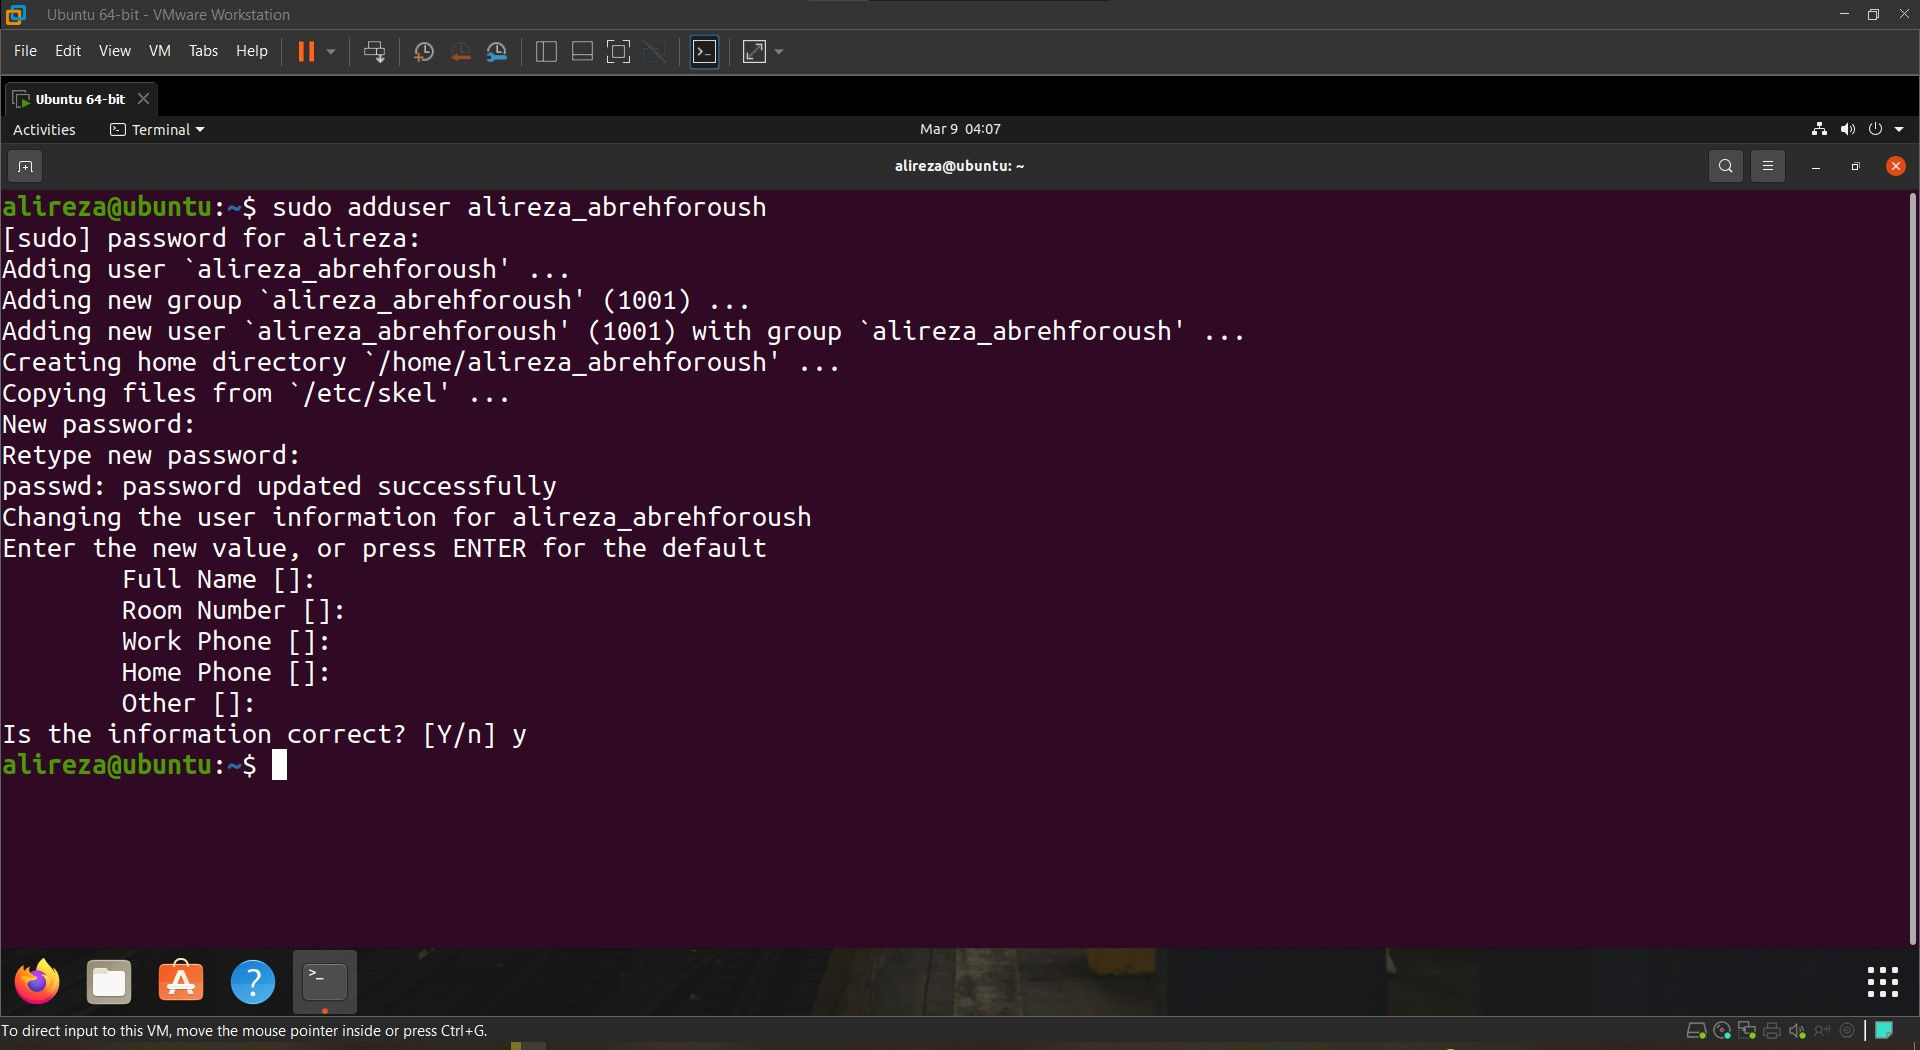
\includegraphics[width=1.0\textwidth]{figures/1a.jpg}
    \caption
	{
\lr{sudo adduser alireza\_abrehforoush}
	}
    \label{fig:fig1}
\end{figure}


\begin{figure}[H]
    \centering
    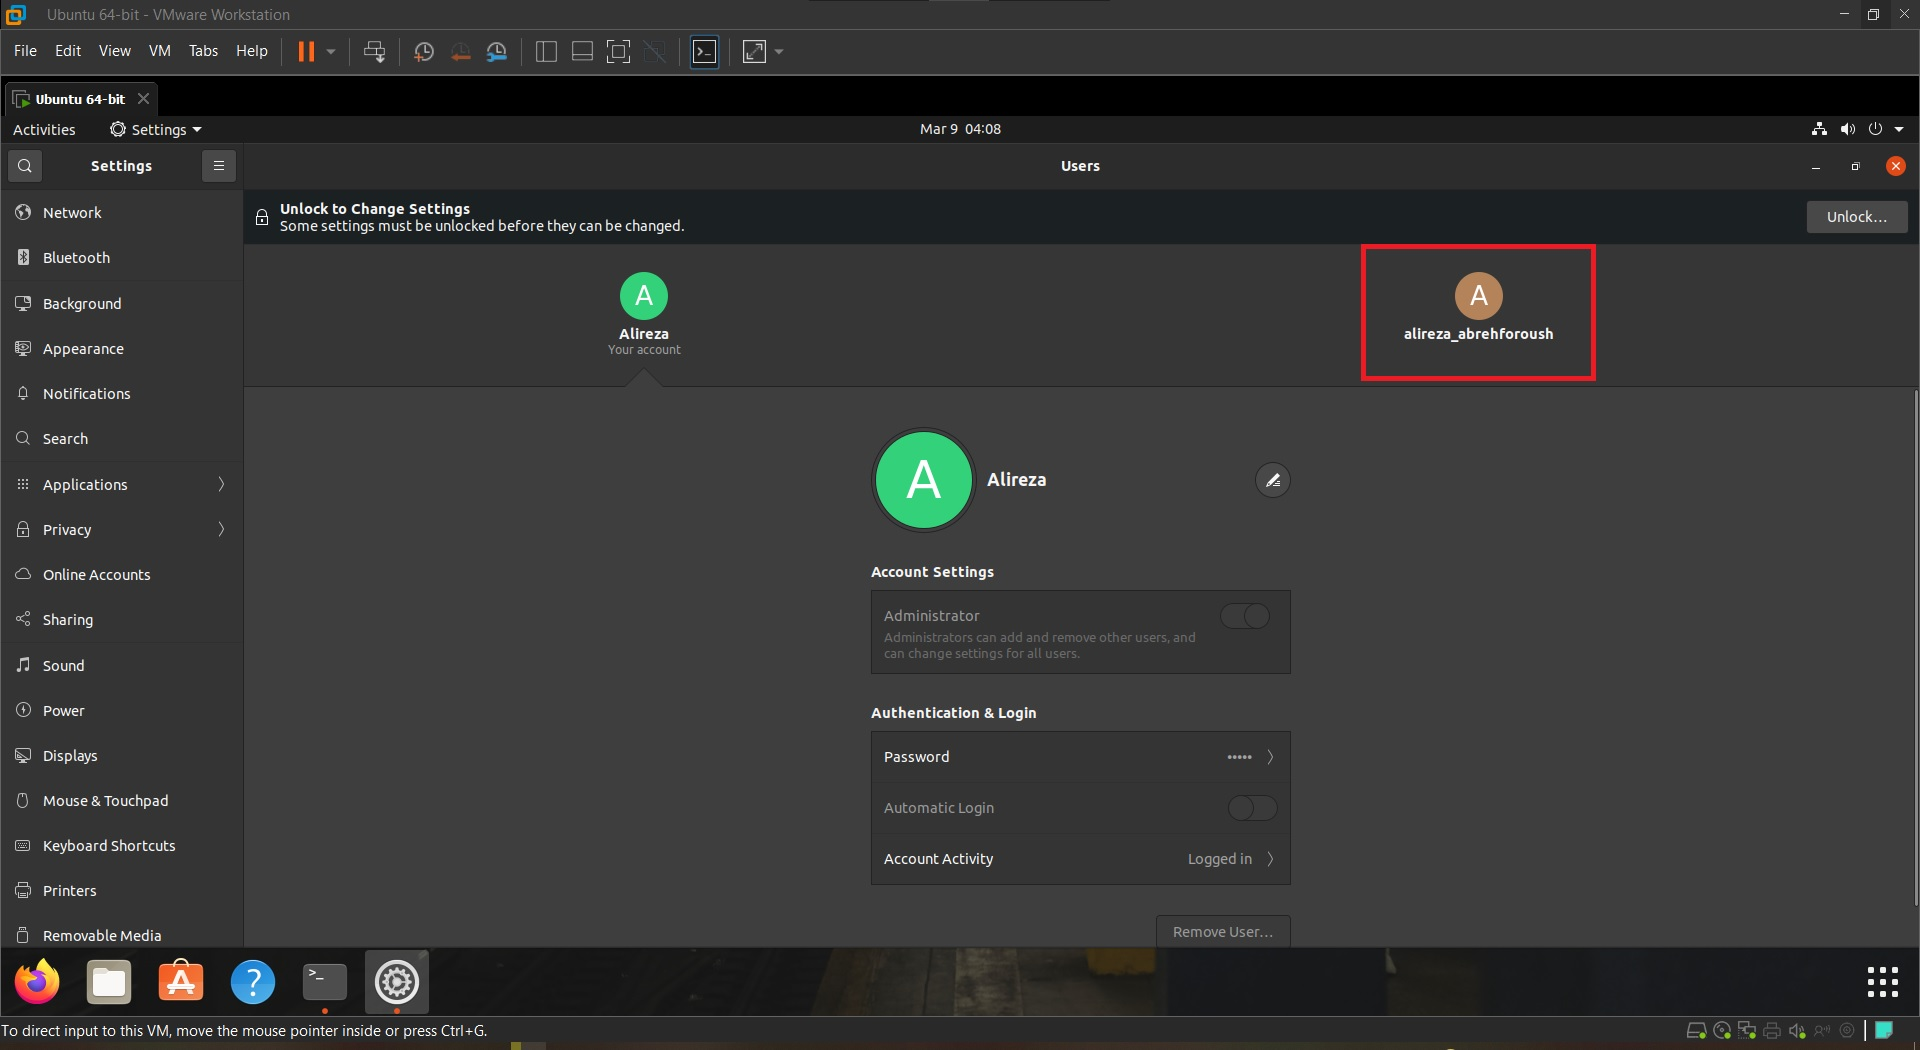
\includegraphics[width=1.0\textwidth]{figures/1b.jpg}
    \caption
	{
\lr{Settings/Users}
	}
    \label{fig:fig1}
\end{figure}
همانطور که در تصویر می‌بینیم، حساب کاربری ایجاد شد.
\section{}
با وارد کردن دستور \lr{sudo su} وارد حالت ریشه می‌شویم.
\begin{figure}[H]
    \centering
    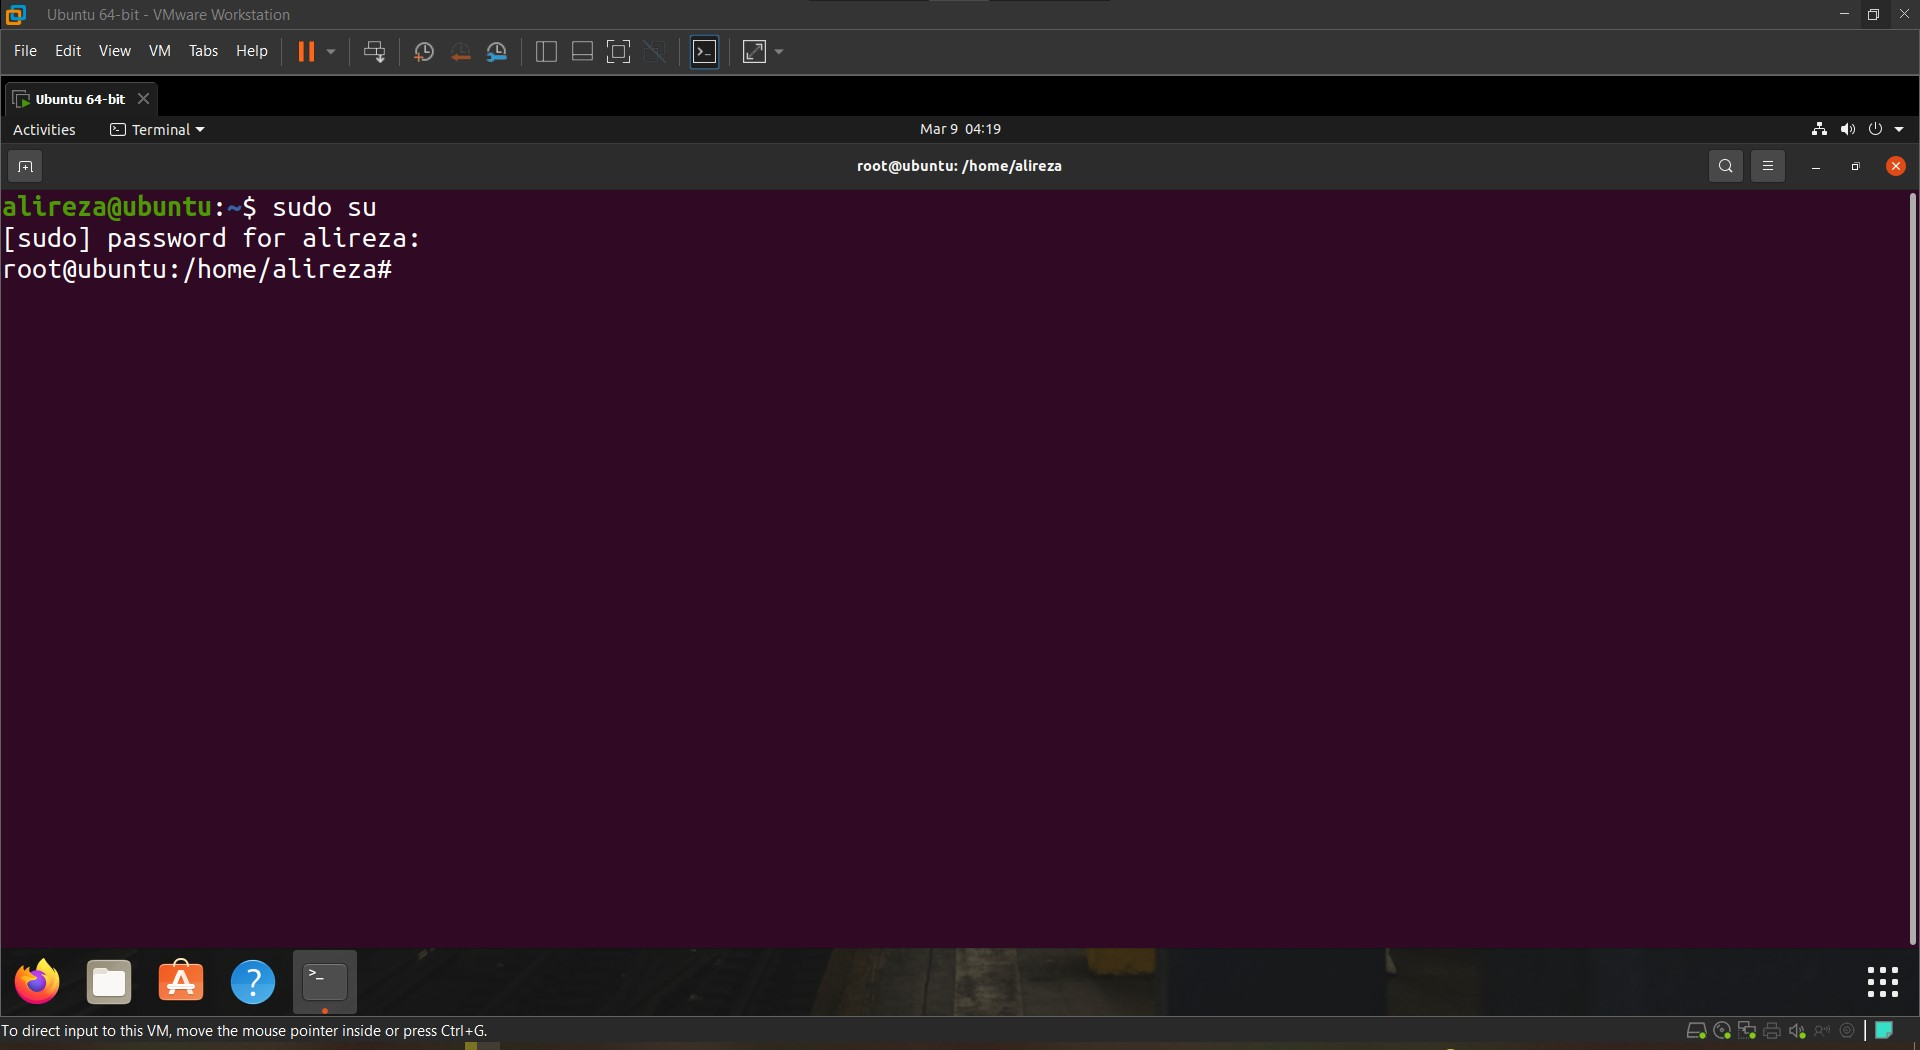
\includegraphics[width=1.0\textwidth]{figures/2.jpg}
    \caption
	{
\lr{sudo su}
	}
    \label{fig:fig1}
\end{figure}

\subsection{تاریخ سیستم}
\begin{figure}[H]
    \centering
    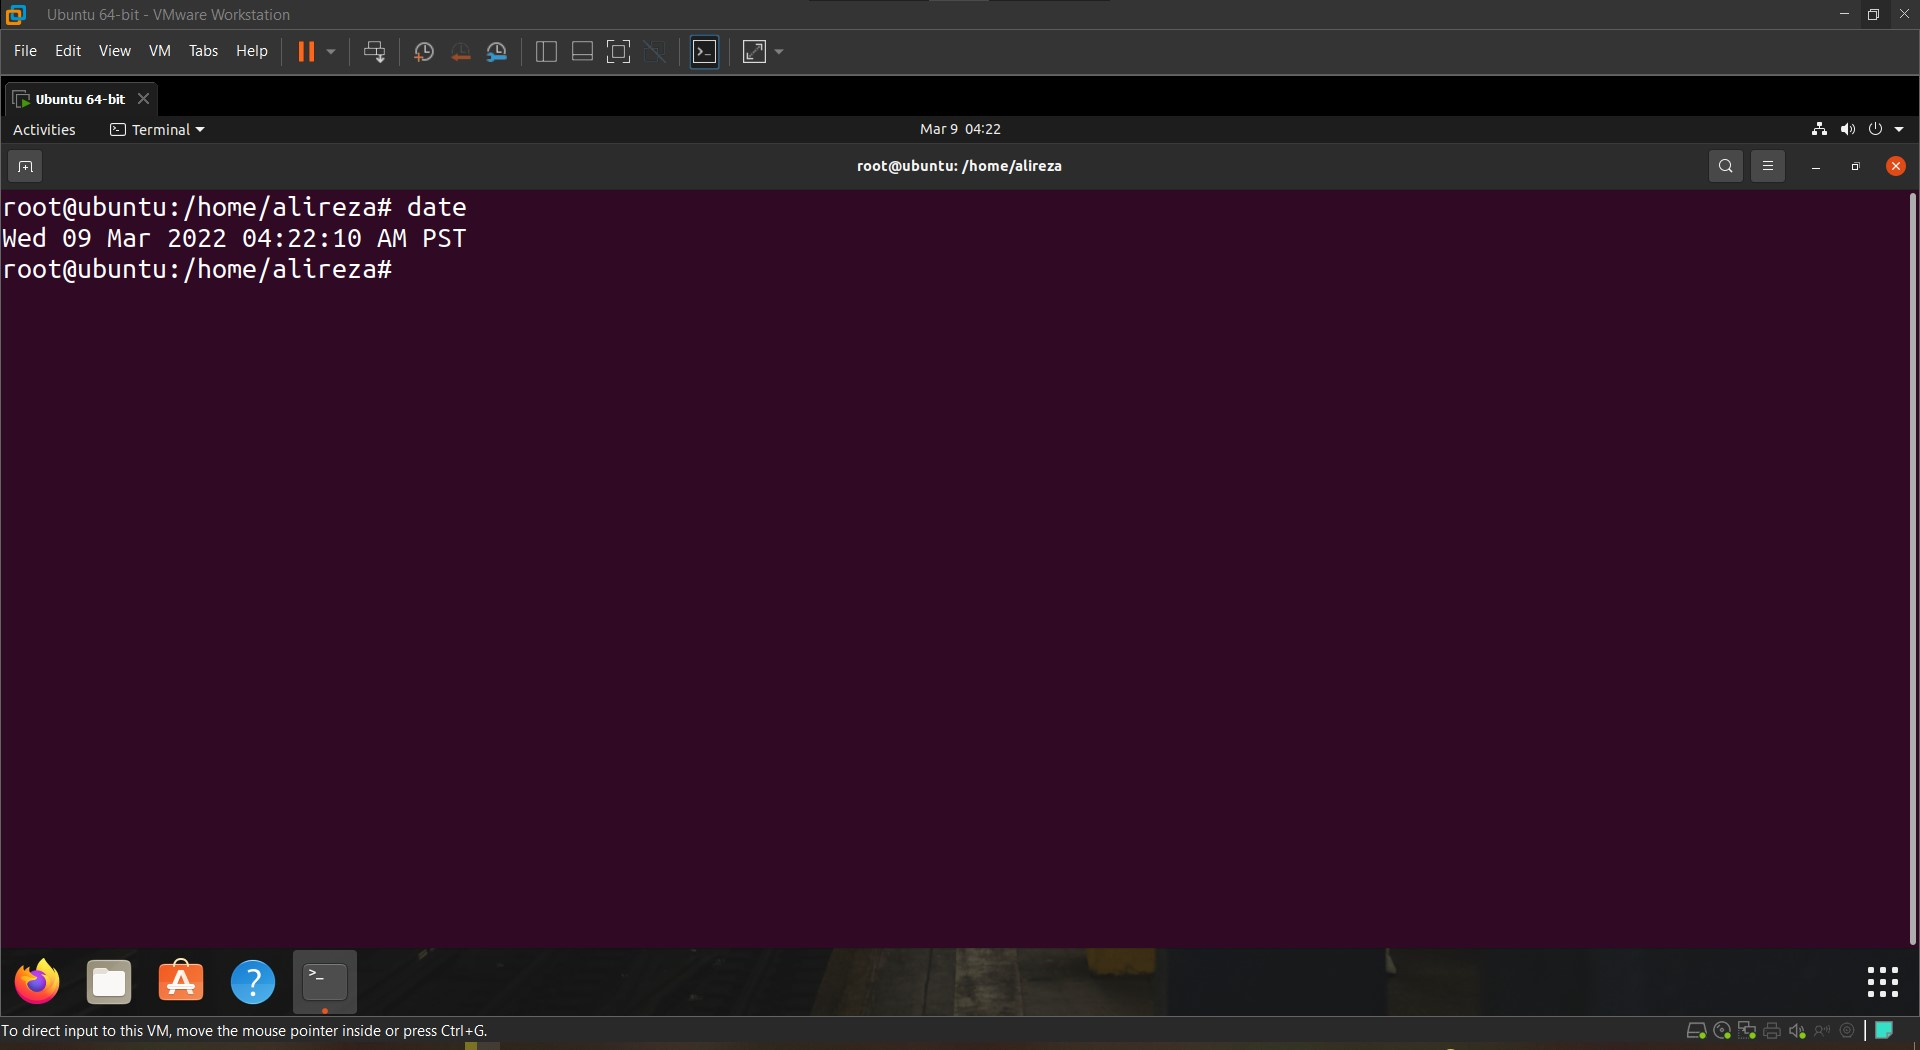
\includegraphics[width=1.0\textwidth]{figures/2a.jpg}
    \caption
	{
\lr{date}
	}
    \label{fig:fig1}
\end{figure}

\subsection{نام سیستم}
\begin{figure}[H]
    \centering
    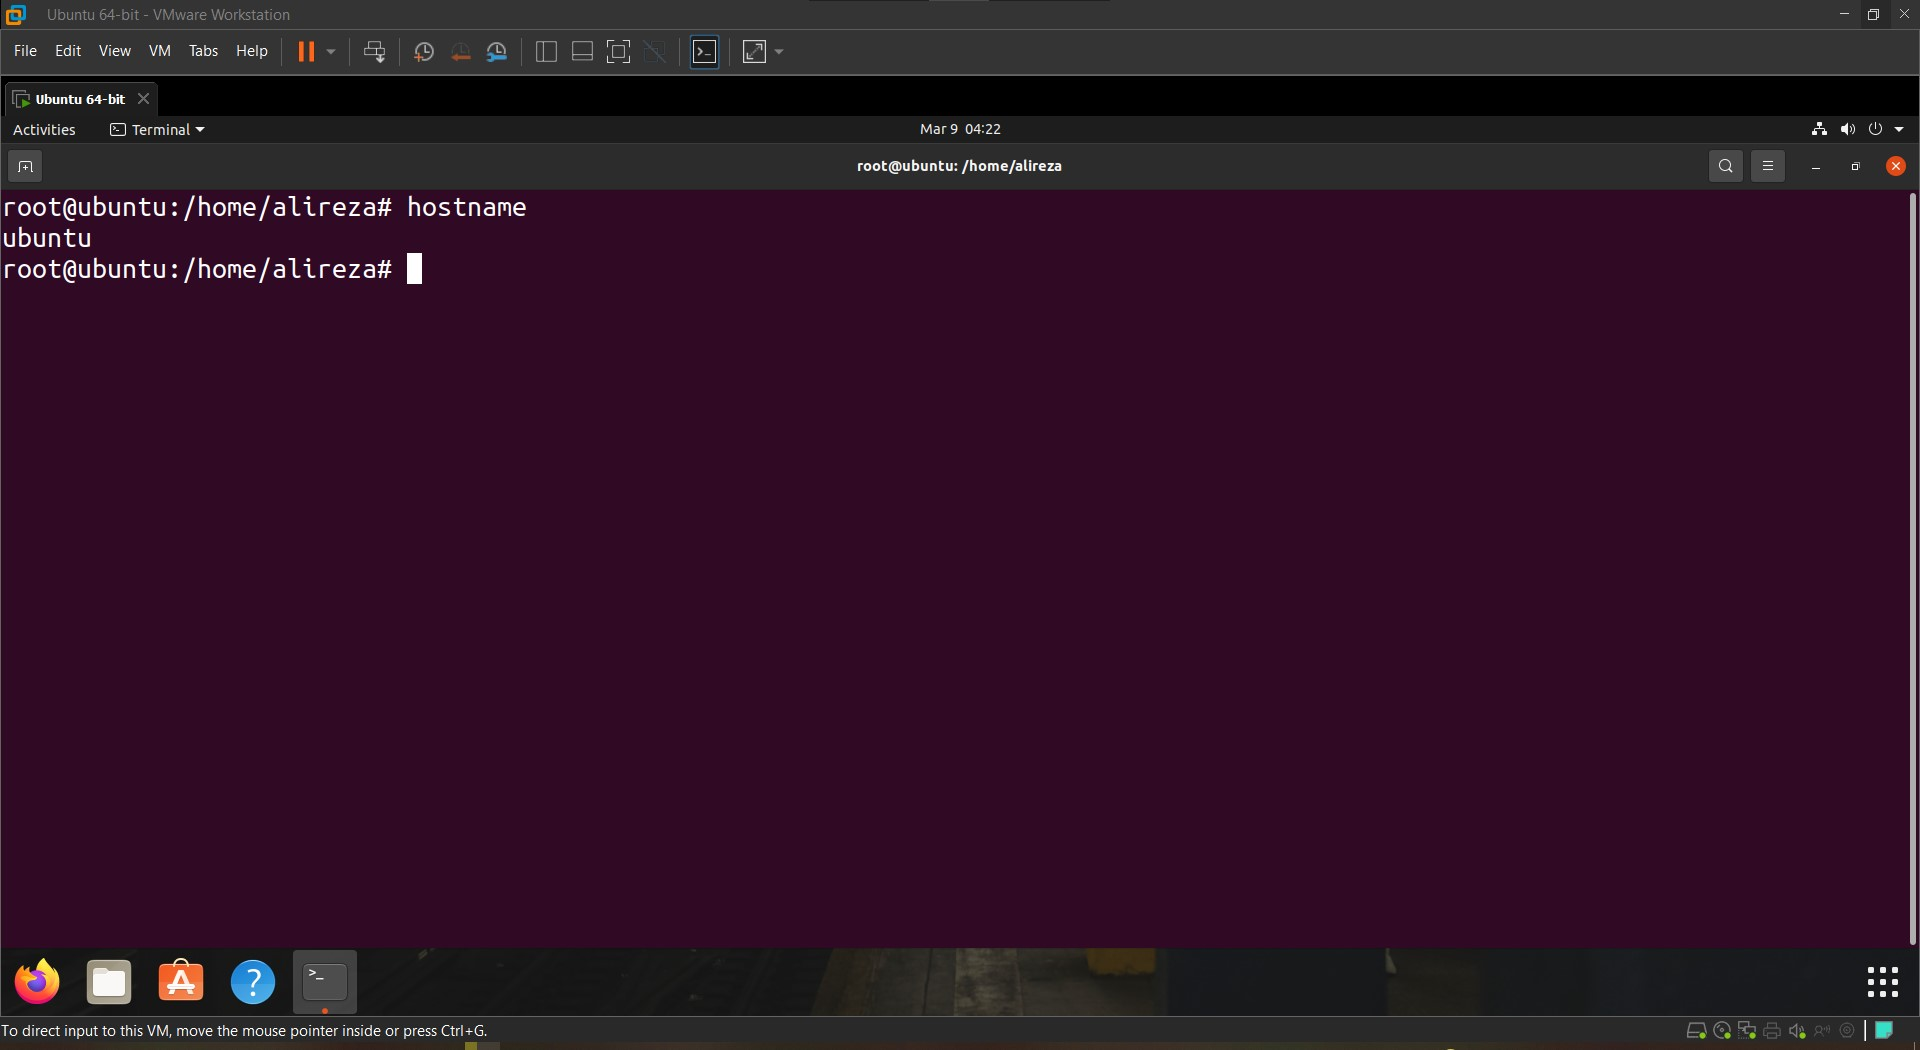
\includegraphics[width=1.0\textwidth]{figures/2b.jpg}
    \caption
	{
\lr{hostname}
	}
    \label{fig:fig1}
\end{figure}

\subsection{نام سیستم‌عامل}
\begin{figure}[H]
    \centering
    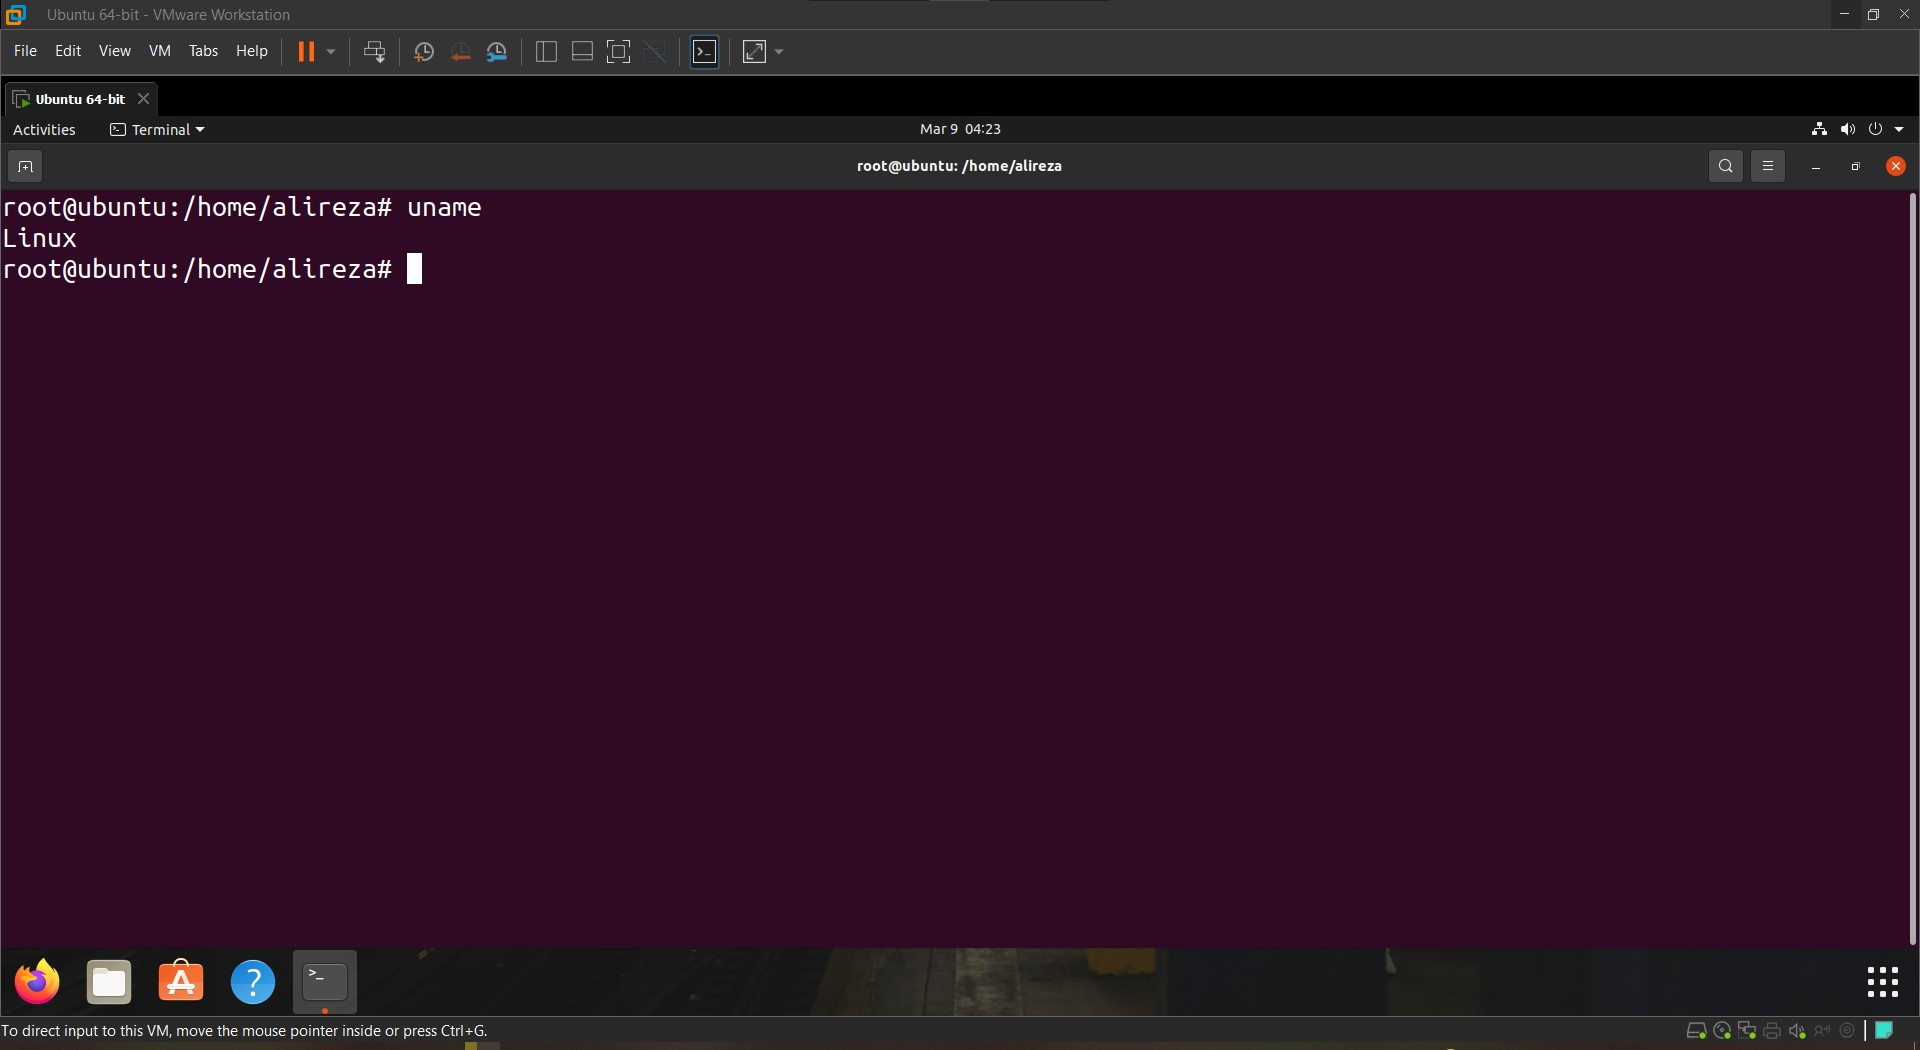
\includegraphics[width=1.0\textwidth]{figures/2c.jpg}
    \caption
	{
\lr{uname}
	}
    \label{fig:fig1}
\end{figure}

\subsection{نام کاربر فعلی}
\begin{figure}[H]
    \centering
    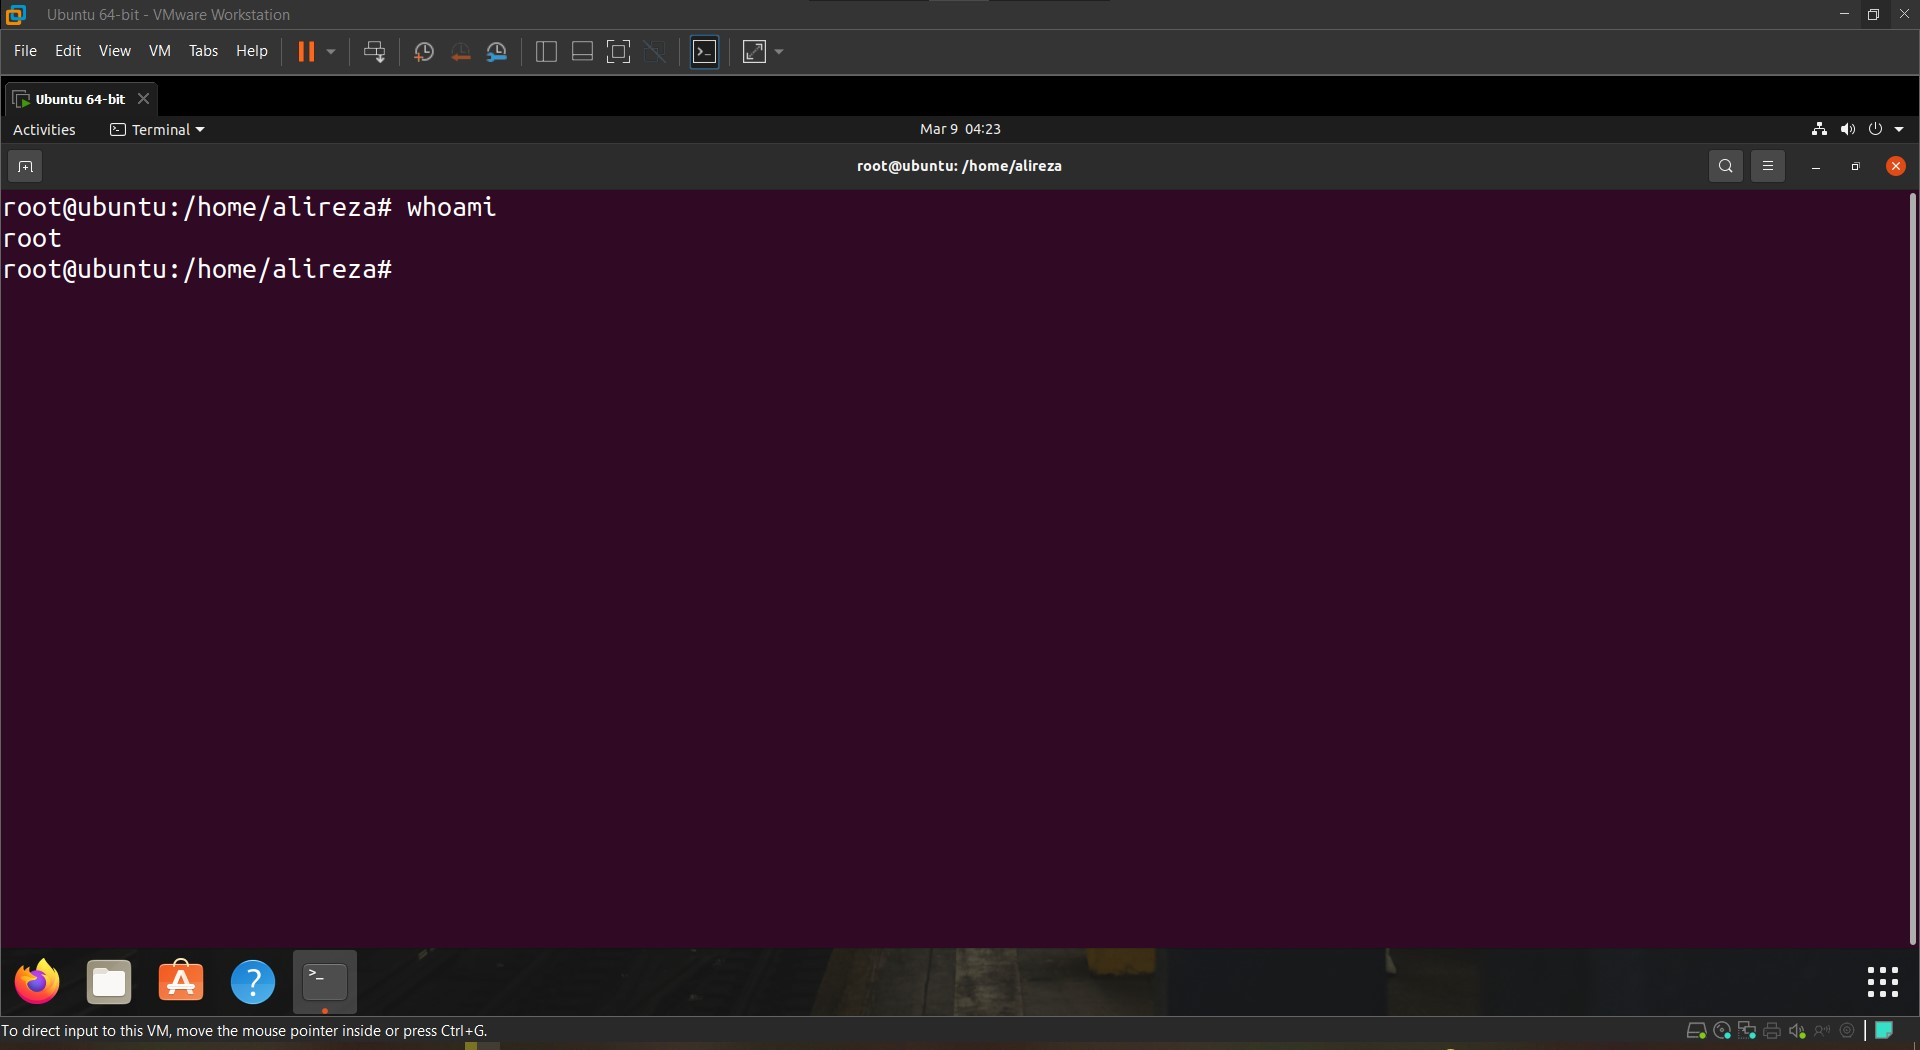
\includegraphics[width=1.0\textwidth]{figures/2d.jpg}
    \caption
	{
\lr{whoami}
	}
    \label{fig:fig1}
\end{figure}

\subsection{پروسه‌های درحال اجرا}
\begin{figure}[H]
    \centering
    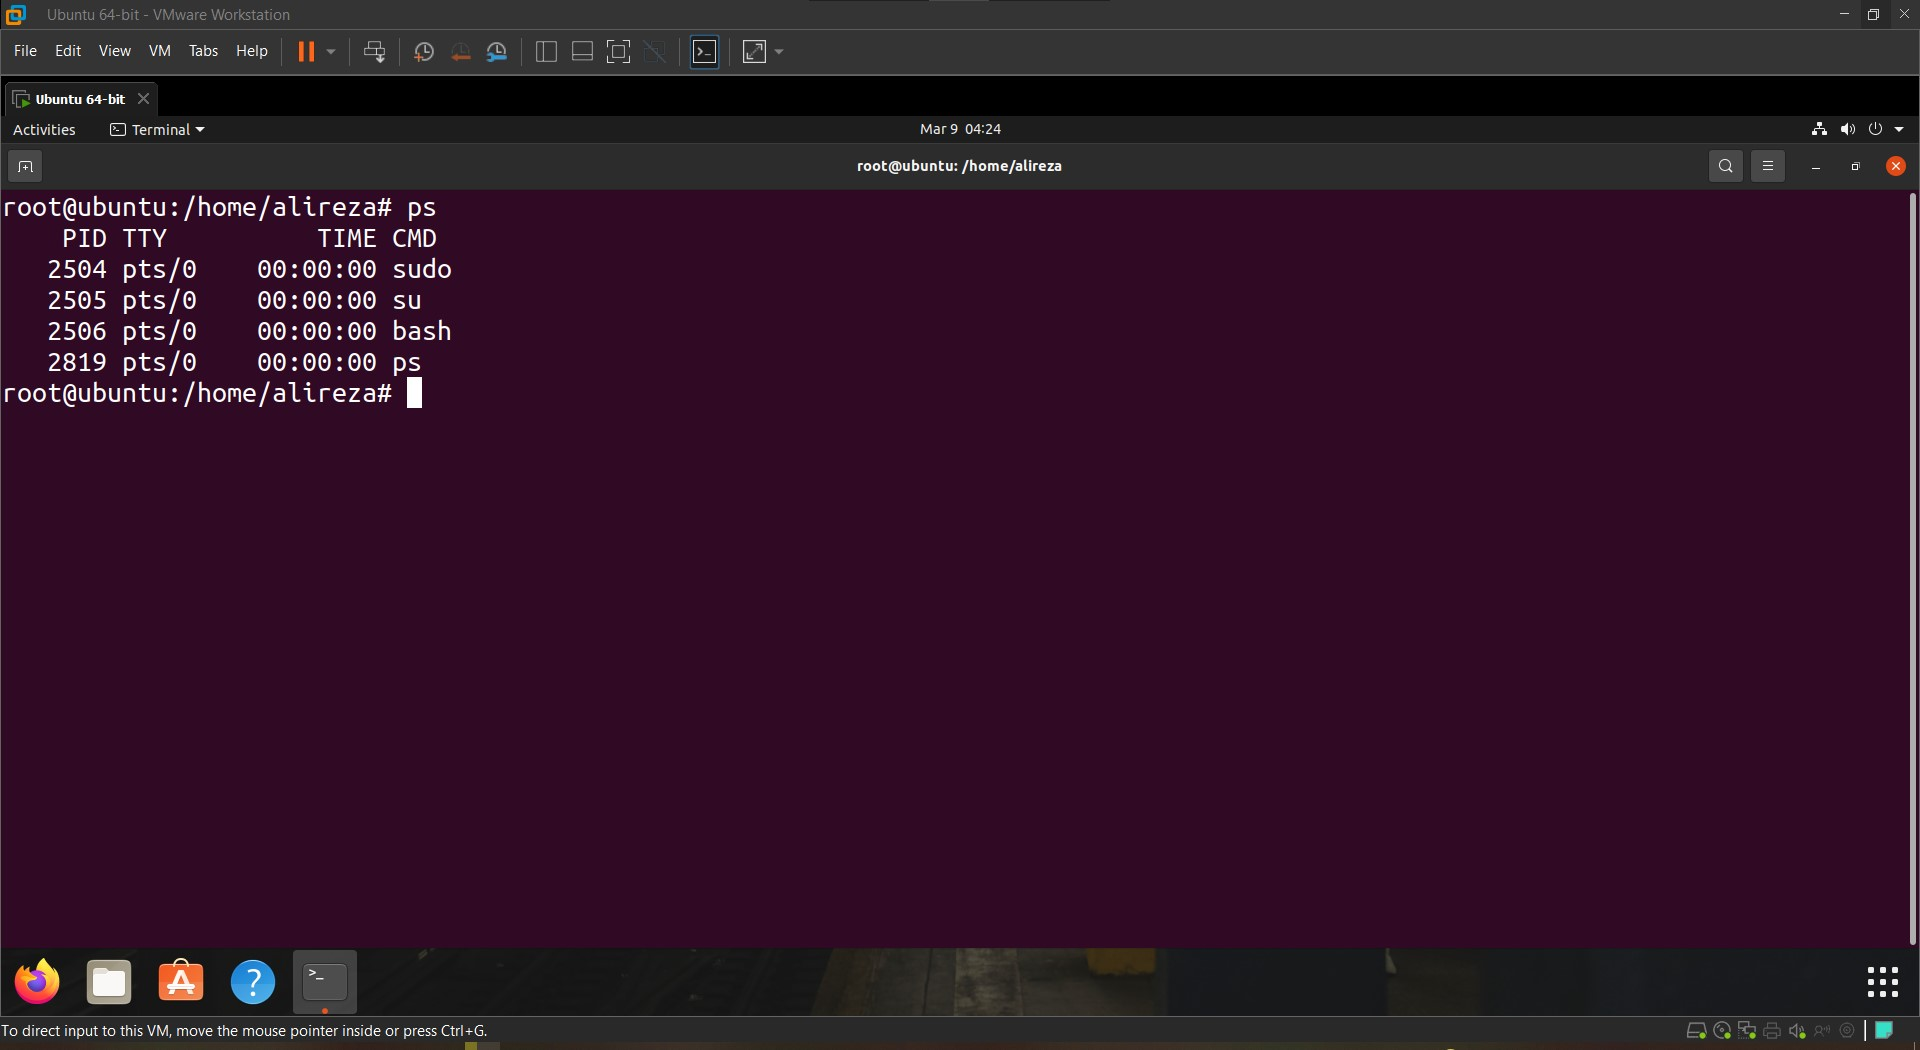
\includegraphics[width=1.0\textwidth]{figures/2e.jpg}
    \caption
	{
\lr{ps}
	}
    \label{fig:fig1}
\end{figure}

\begin{latin}

PID: Every process is assigned a PID (Process Identifier) which is a unique identifier that is associated with a running process in the system.

TTY: Controlling terminal associated with the process.

STAT: Process State Code

TIME: Total time of CPU Usage

CMD: The command that is executed by the process.
\end{latin}


\section{کار با دایرکتوری‌ها}

\subsection{}
\begin{figure}[H]
    \centering
    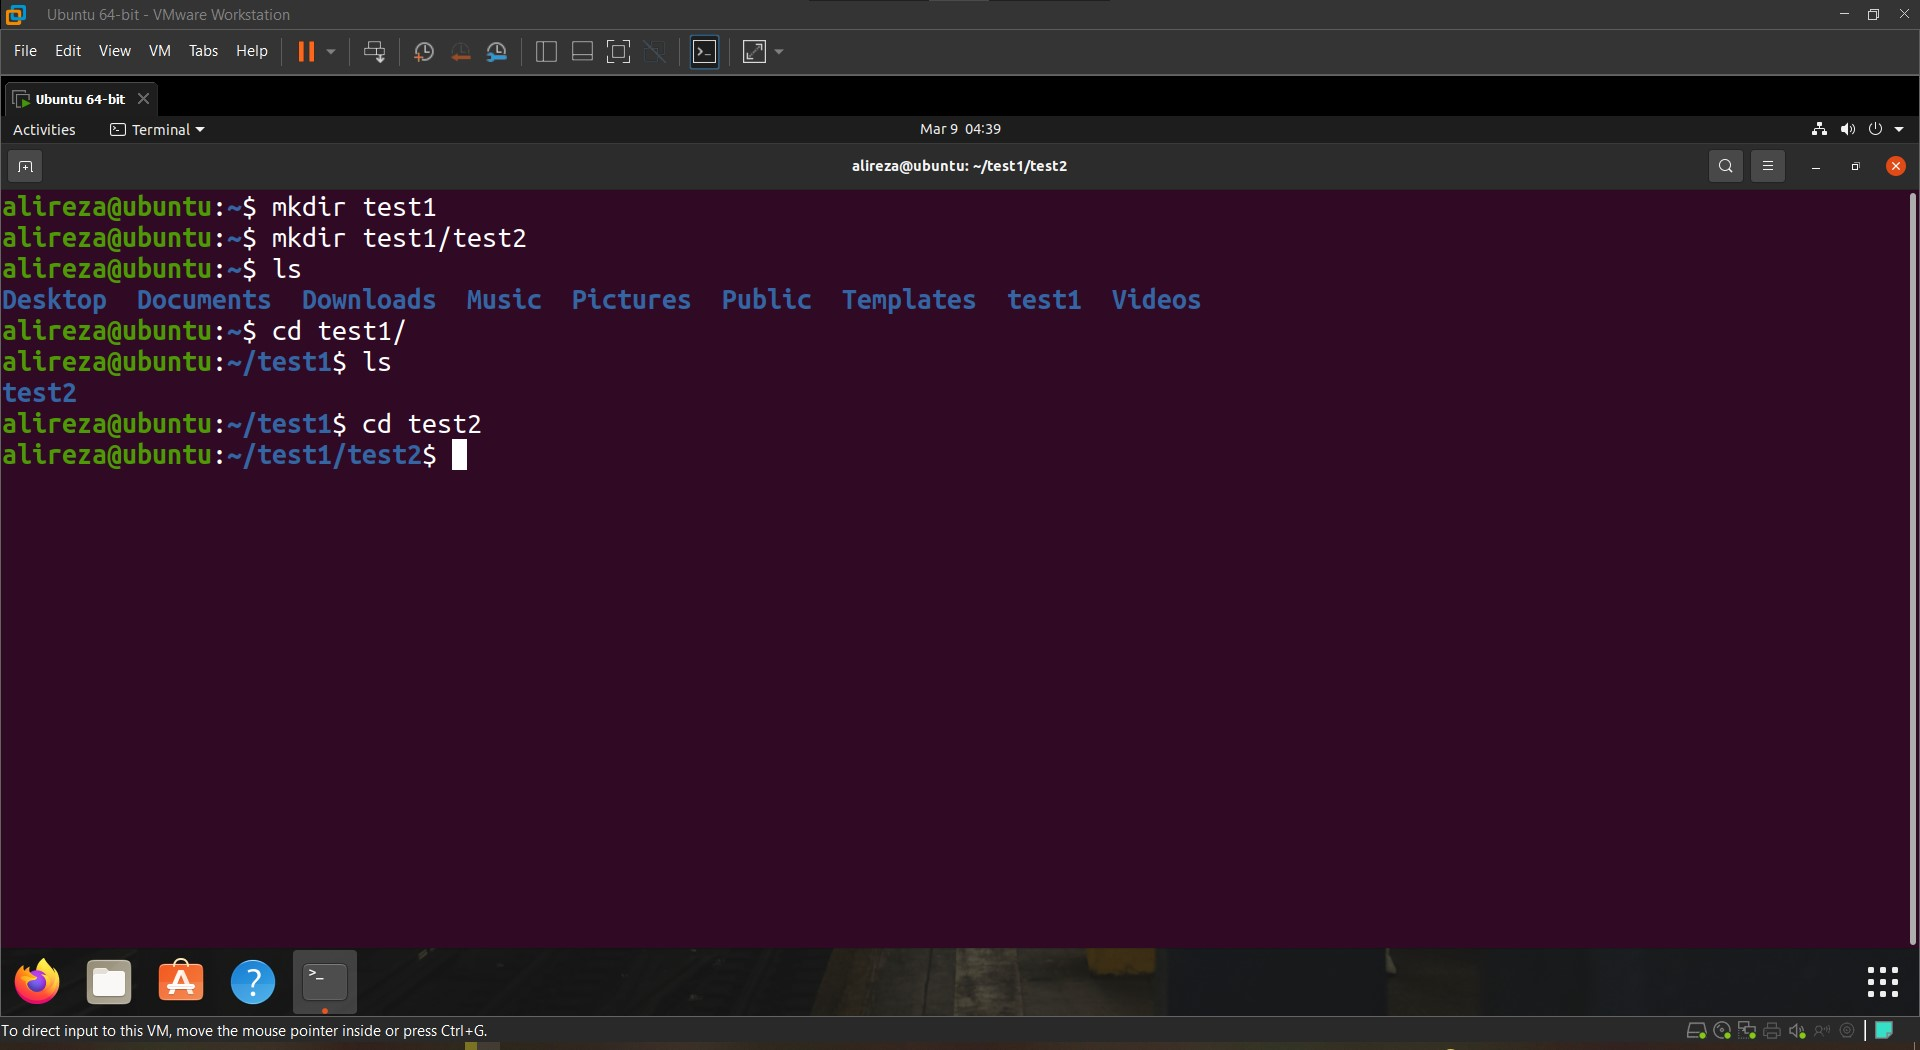
\includegraphics[width=1.0\textwidth]{figures/3a.jpg}
    \caption
	{
\lr{a}
	}
    \label{fig:fig1}
\end{figure}

\subsection{}
\begin{figure}[H]
    \centering
    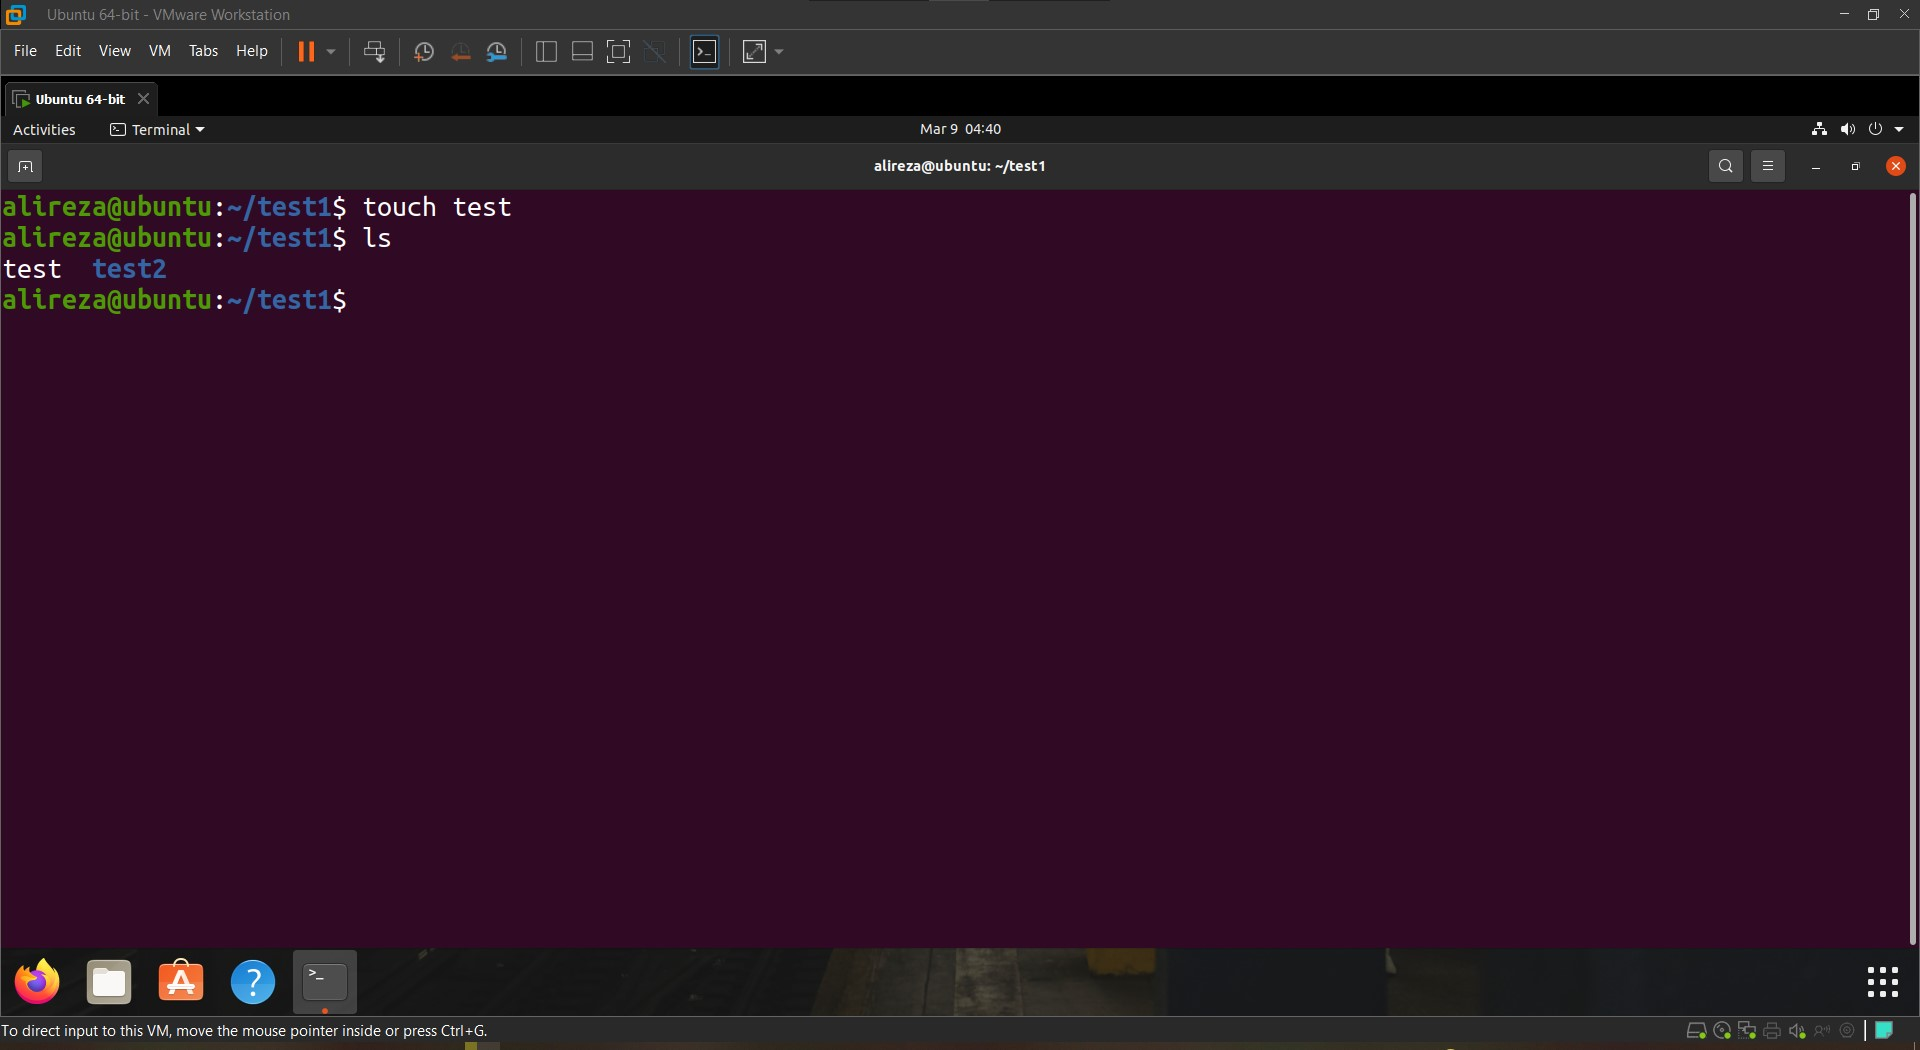
\includegraphics[width=1.0\textwidth]{figures/3b.jpg}
    \caption
	{
\lr{b}
	}
    \label{fig:fig1}
\end{figure}

\subsection{}
\begin{figure}[H]
    \centering
    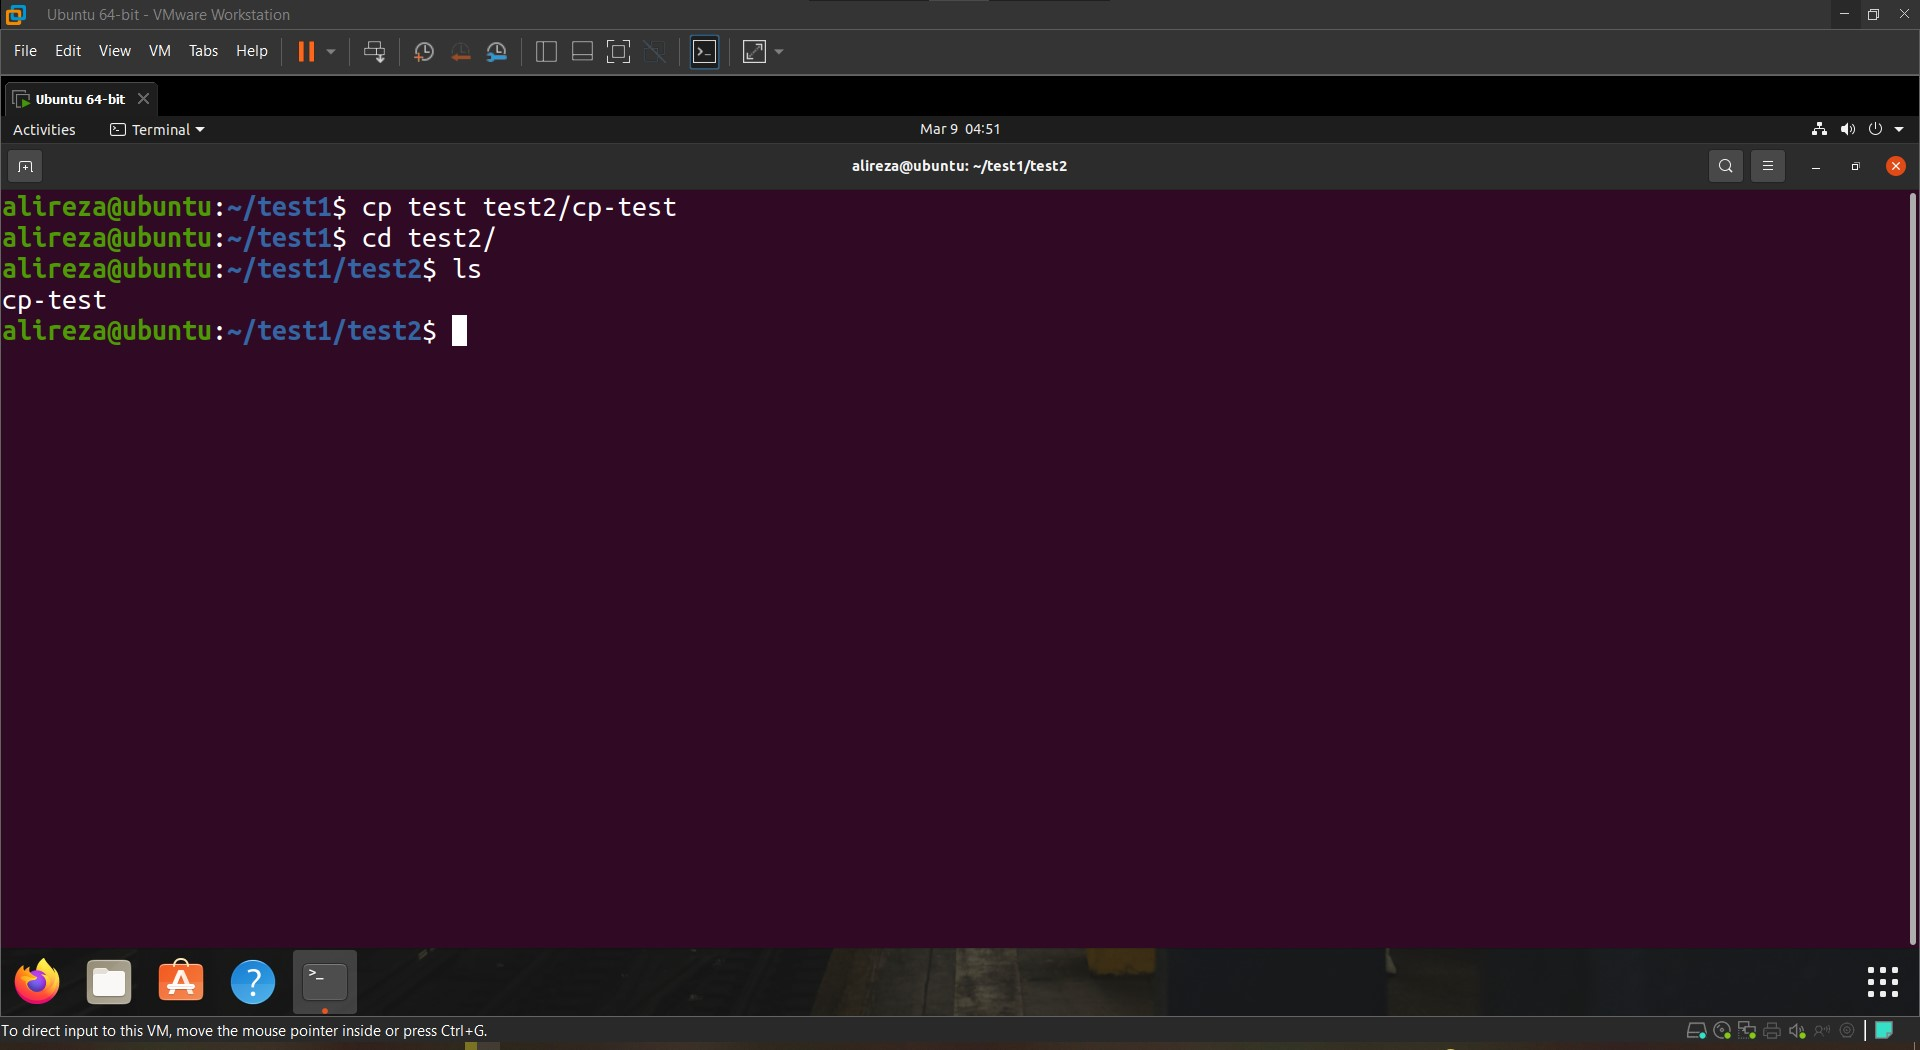
\includegraphics[width=1.0\textwidth]{figures/3c.jpg}
    \caption
	{
\lr{c}
	}
    \label{fig:fig1}
\end{figure}

\subsection{}
\begin{figure}[H]
    \centering
    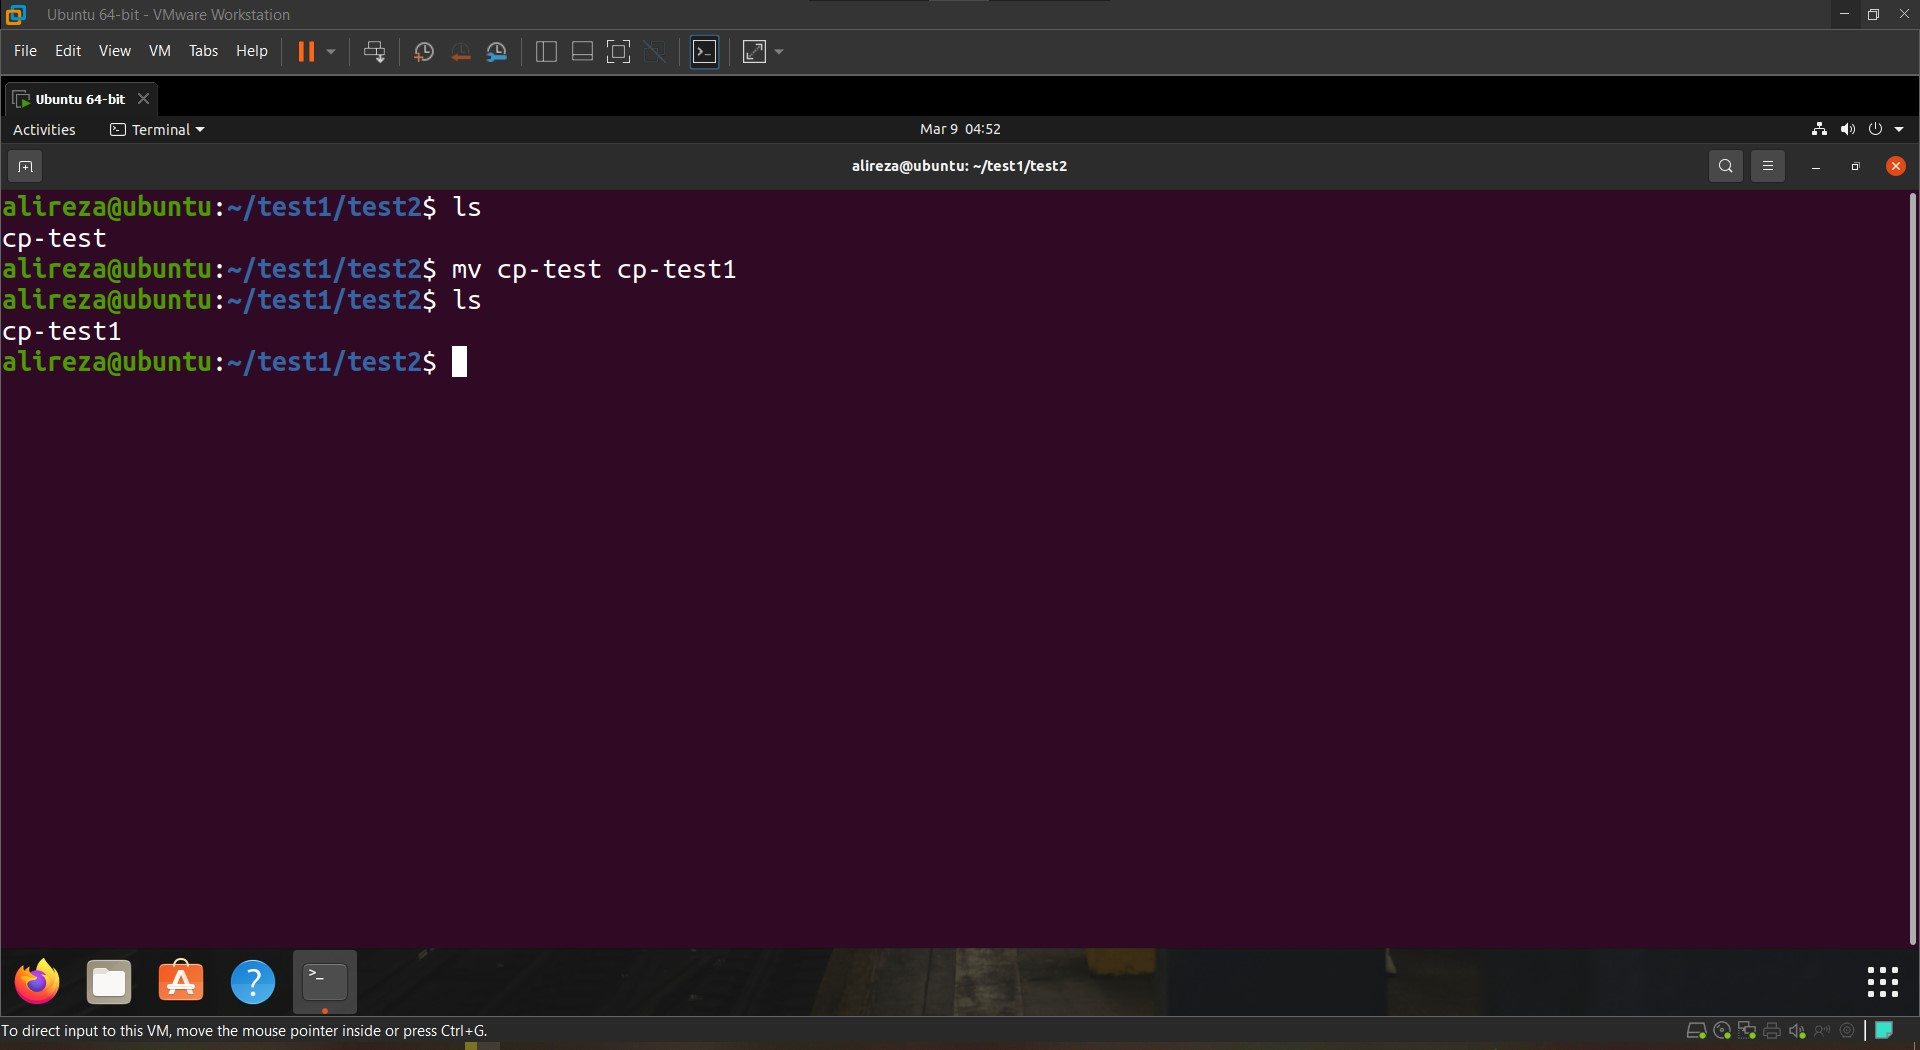
\includegraphics[width=1.0\textwidth]{figures/3d.jpg}
    \caption
	{
\lr{d}
	}
    \label{fig:fig1}
\end{figure}

\subsection{}
\begin{figure}[H]
    \centering
    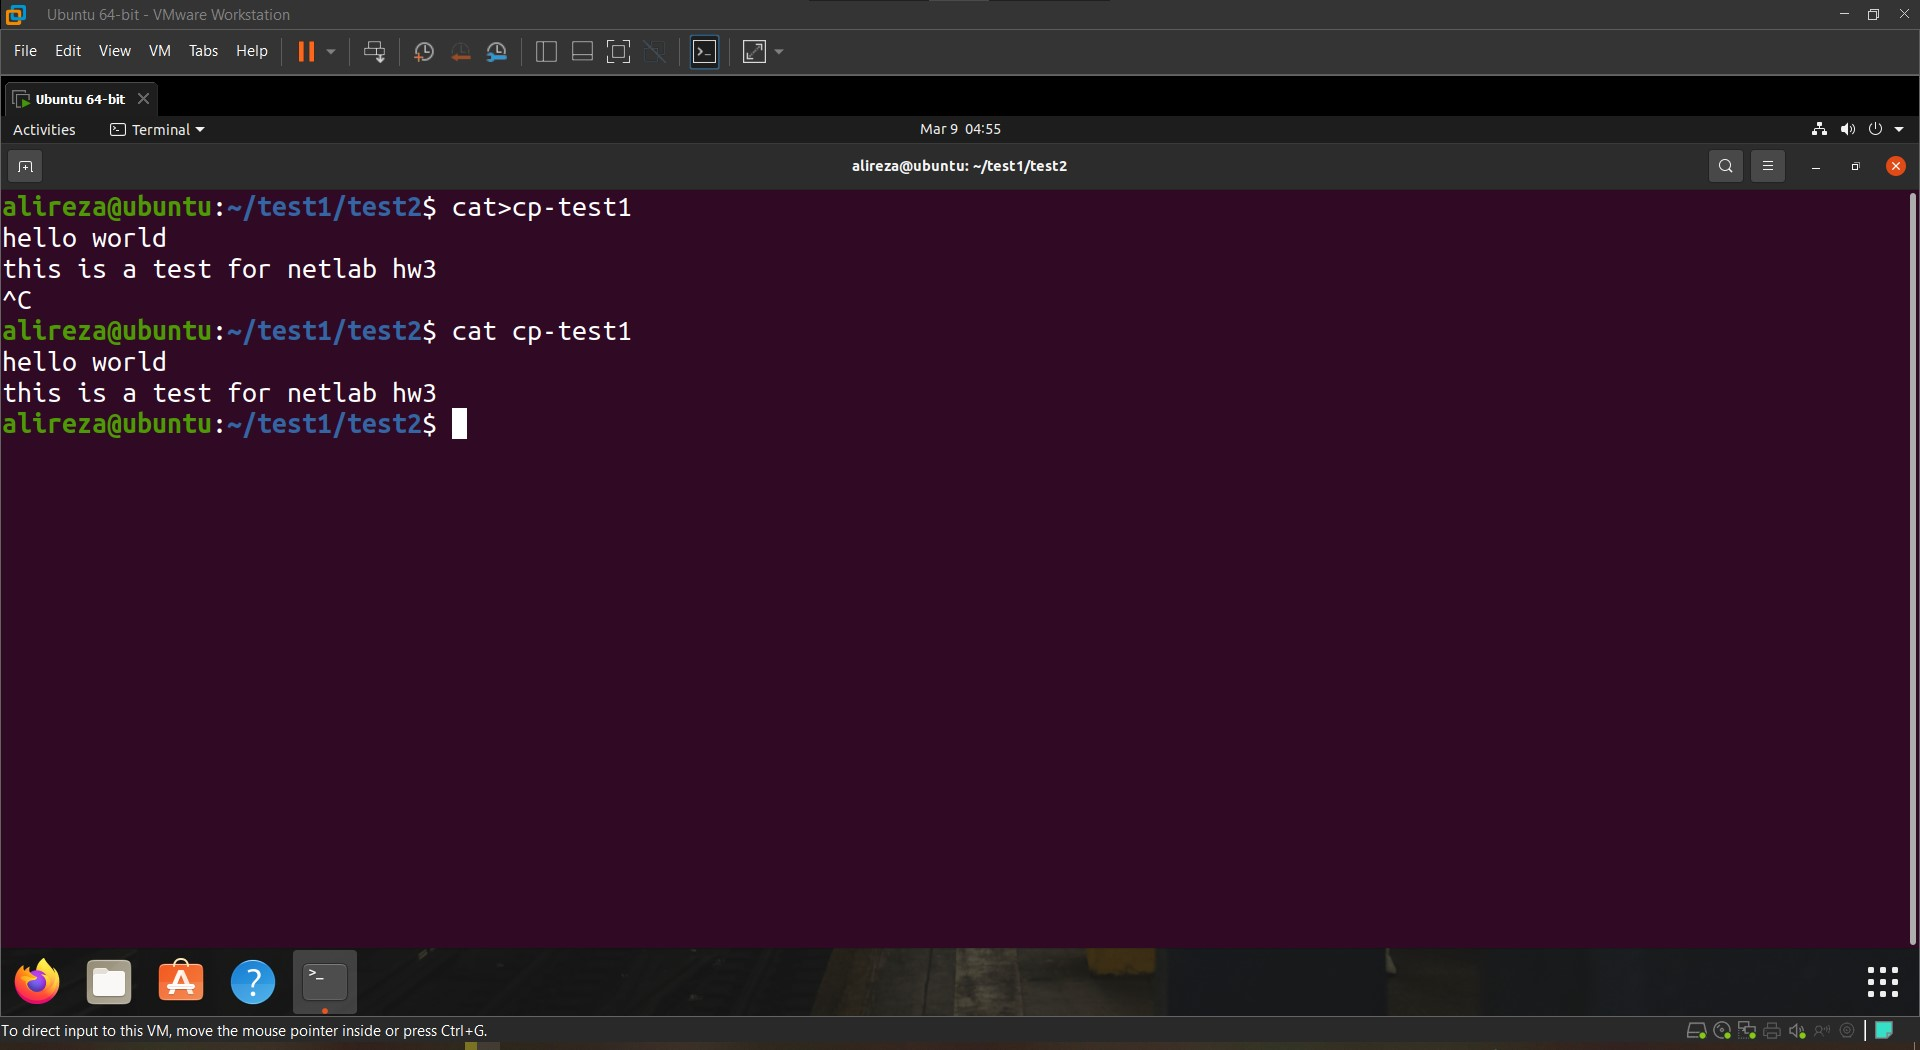
\includegraphics[width=1.0\textwidth]{figures/3e.jpg}
    \caption
	{
\lr{e}
	}
    \label{fig:fig1}
\end{figure}

\subsection{}
\begin{figure}[H]
    \centering
    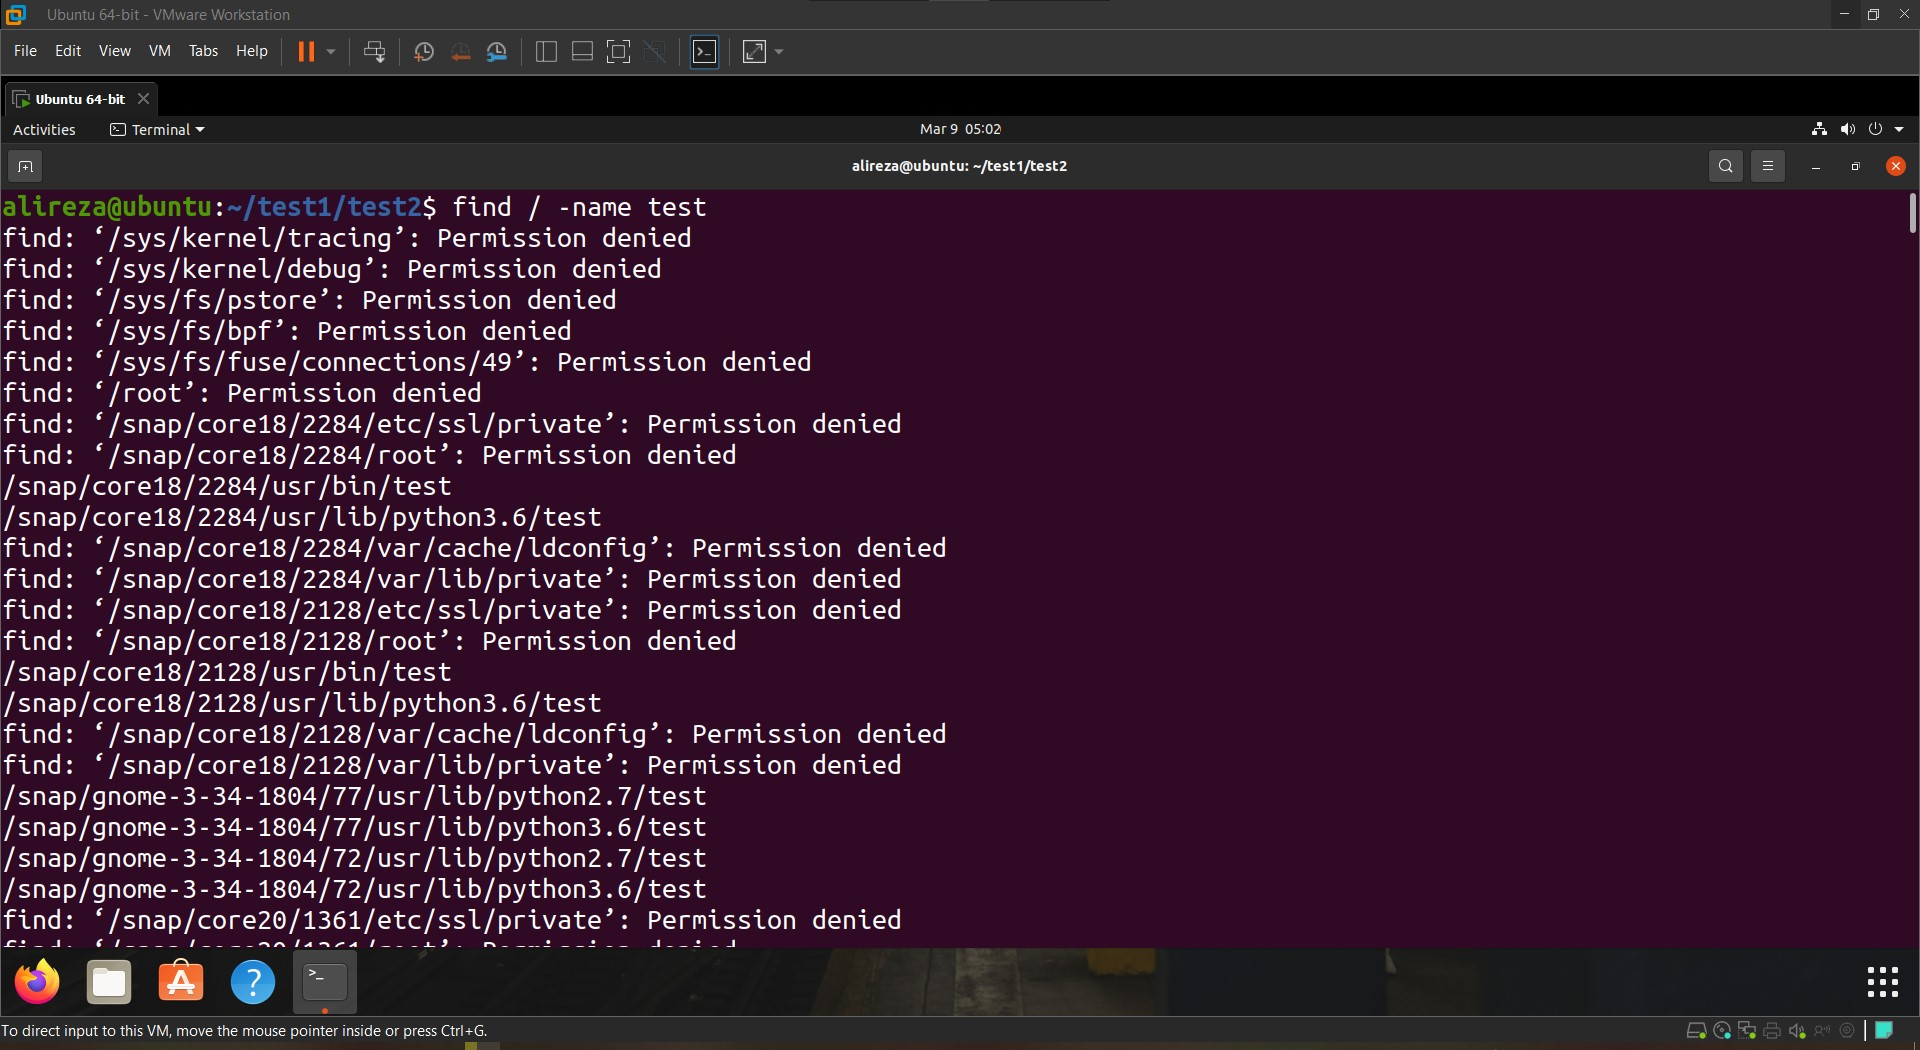
\includegraphics[width=1.0\textwidth]{figures/3f.jpg}
    \caption
	{
\lr{f}
	}
    \label{fig:fig1}
\end{figure}




\section{کار با ویرایشگر \lr{vi}}
\begin{figure}[H]
    \centering
    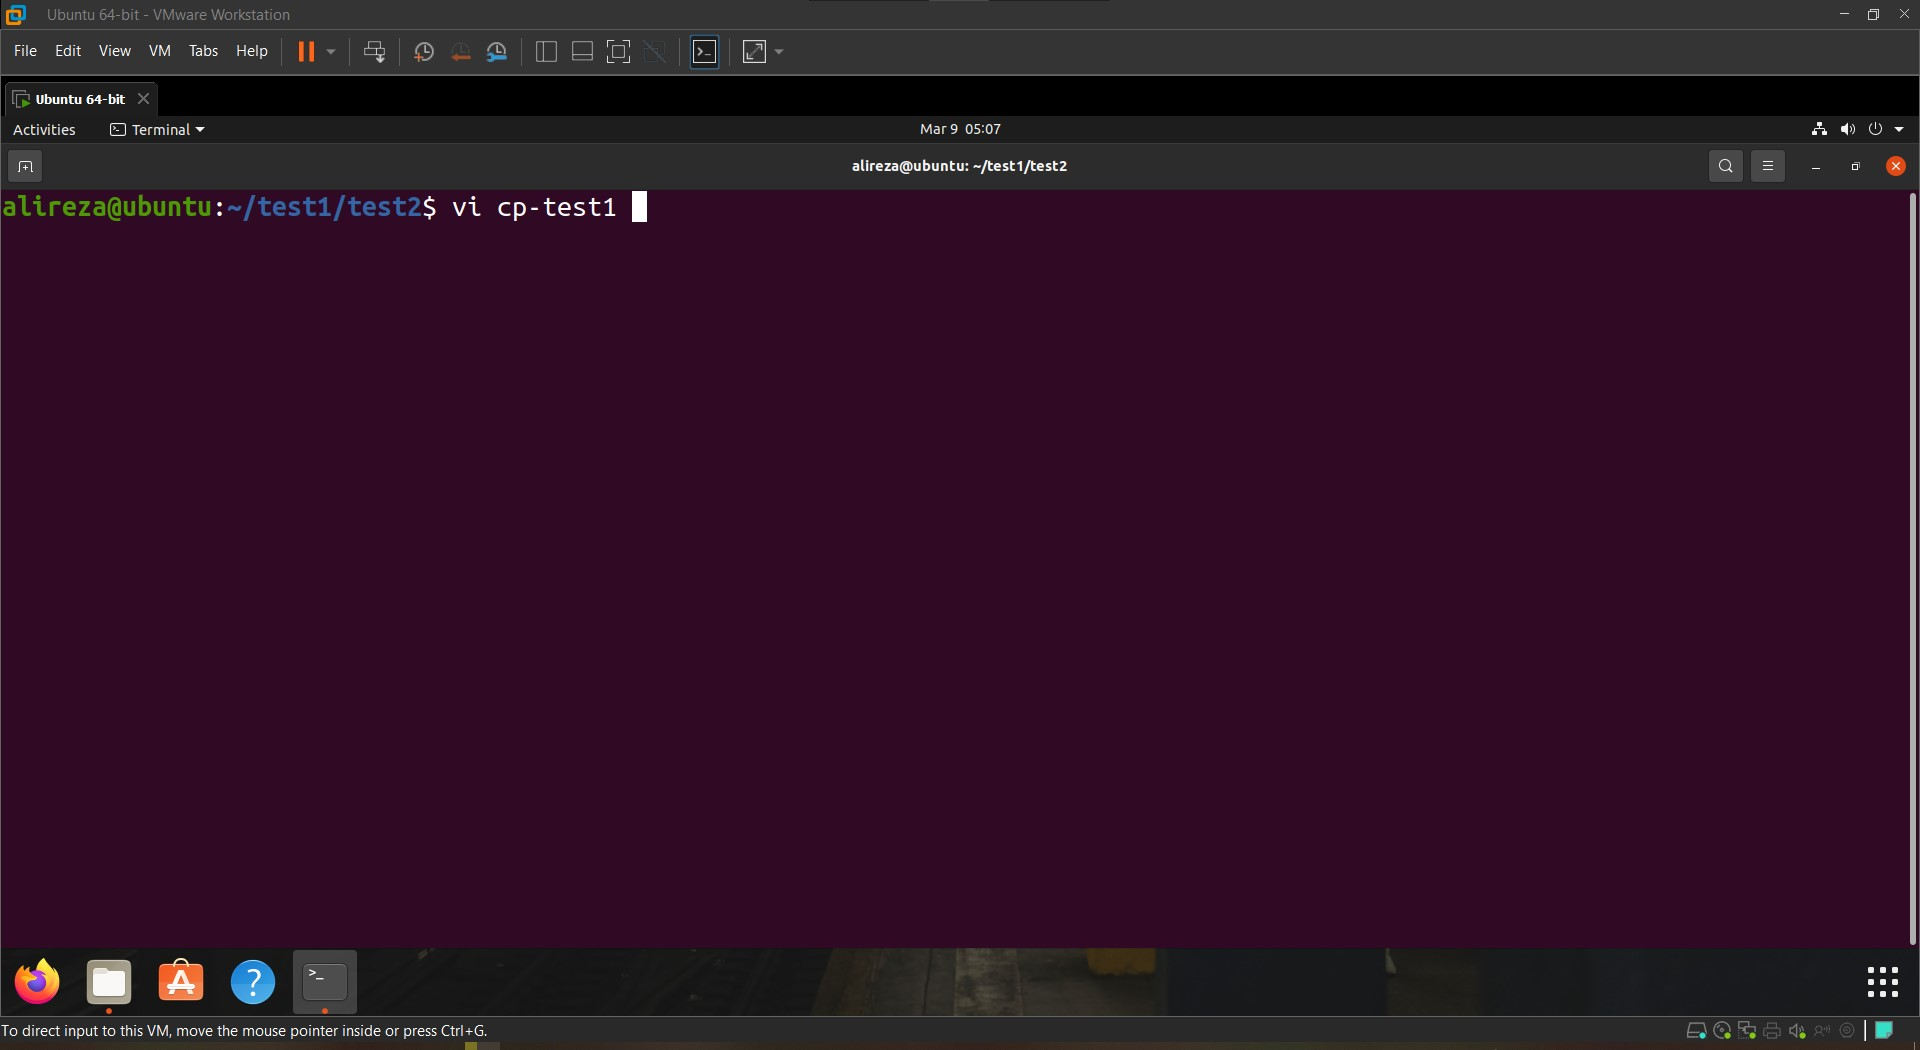
\includegraphics[width=1.0\textwidth]{figures/4a1.jpg}
    \caption
	{
بازکردن فایل برای ویرایش
	}
    \label{fig:fig1}
\end{figure}

\begin{figure}[H]
    \centering
    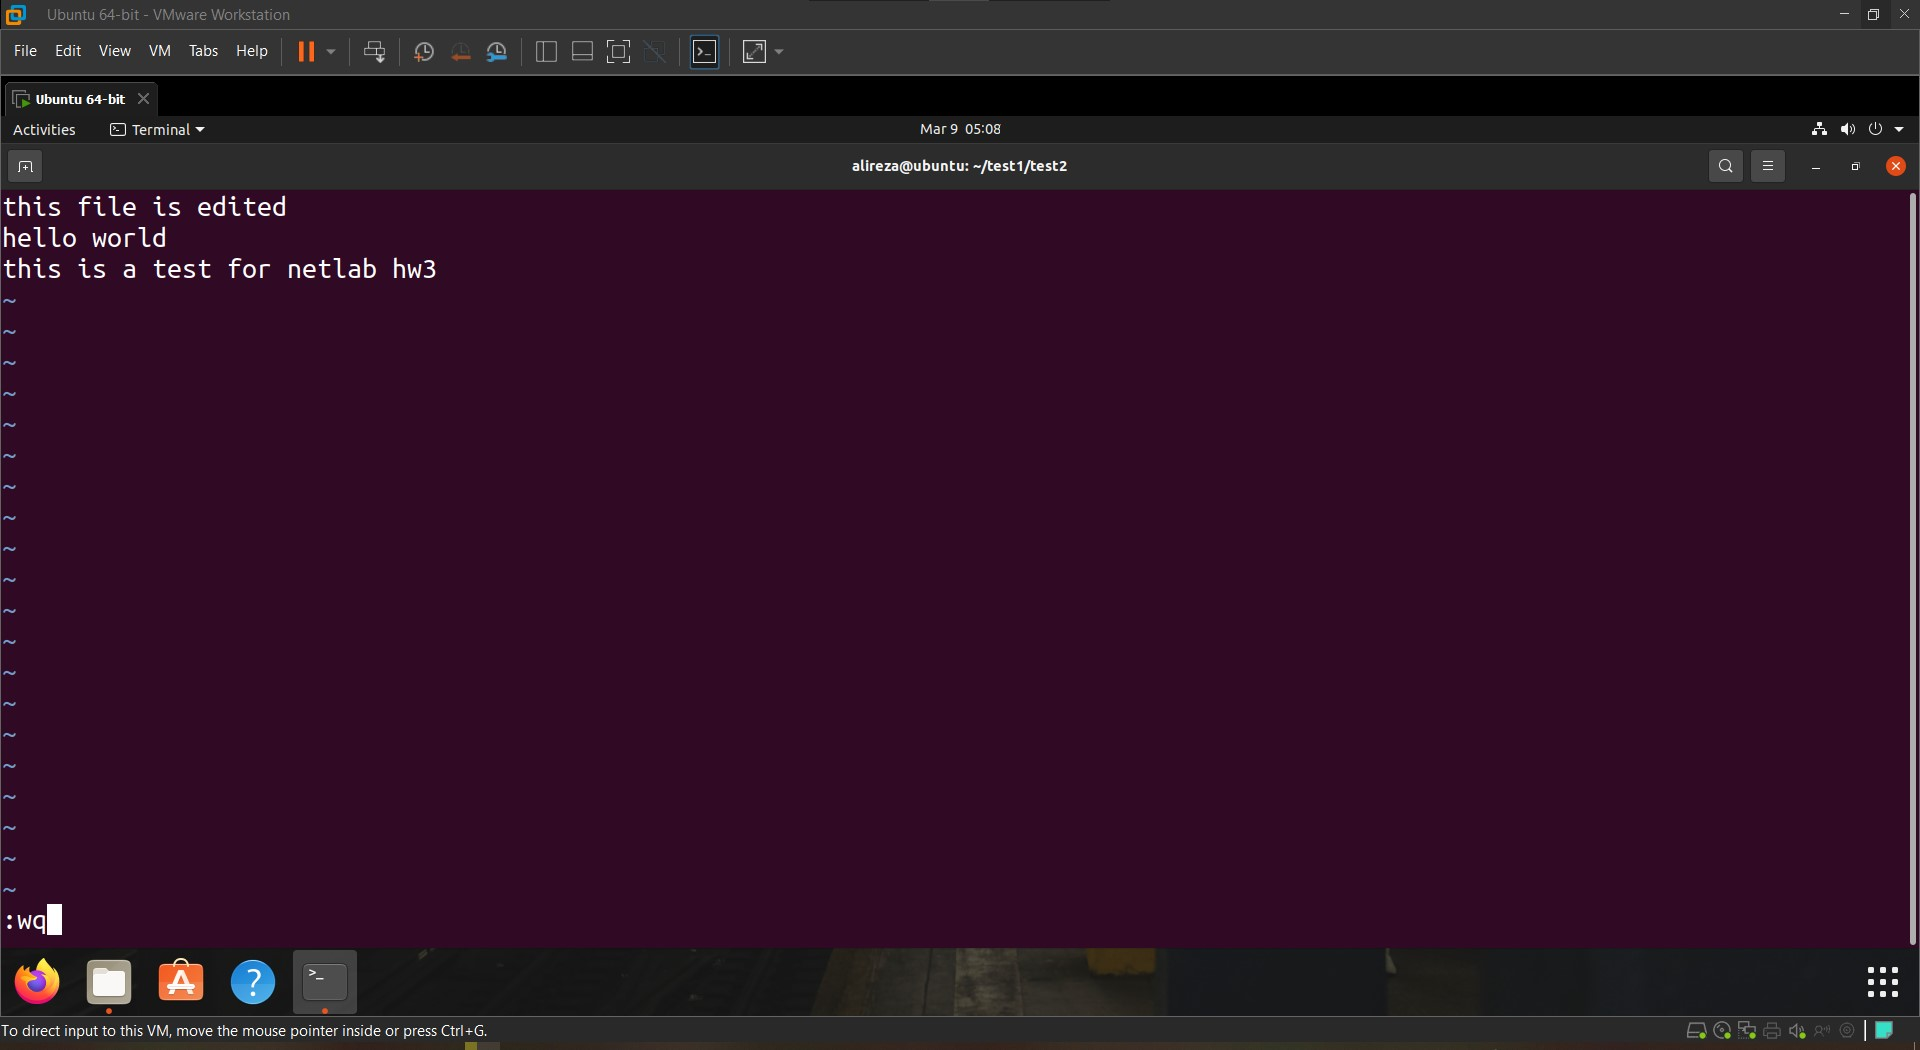
\includegraphics[width=1.0\textwidth]{figures/4a2.jpg}
    \caption
	{
ویرایش فایل
	}
    \label{fig:fig1}
\end{figure}

\begin{figure}[H]
    \centering
    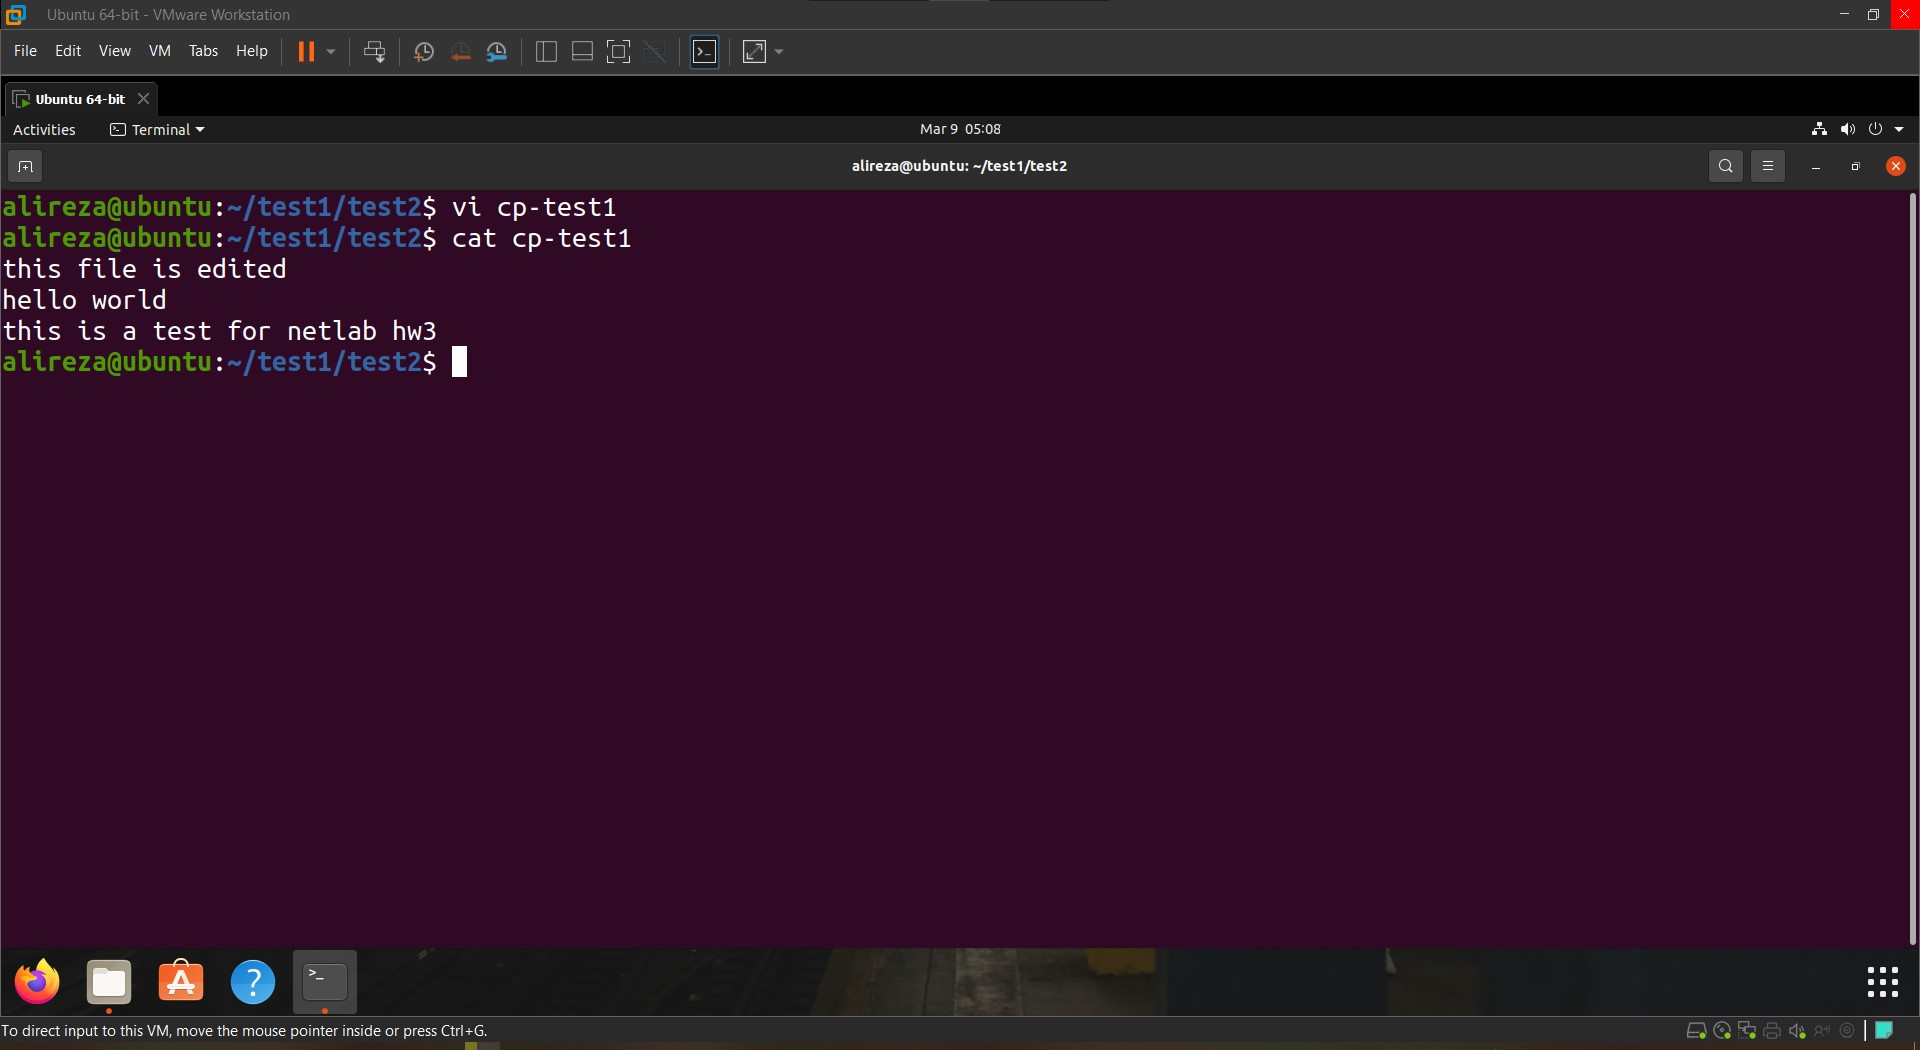
\includegraphics[width=1.0\textwidth]{figures/4a3.jpg}
    \caption
	{
خروجی فایل ویرایش شده
	}
    \label{fig:fig1}
\end{figure}

\section{تغییر نوع دسترسی به فایل}
\subsection{}
\begin{figure}[H]
    \centering
    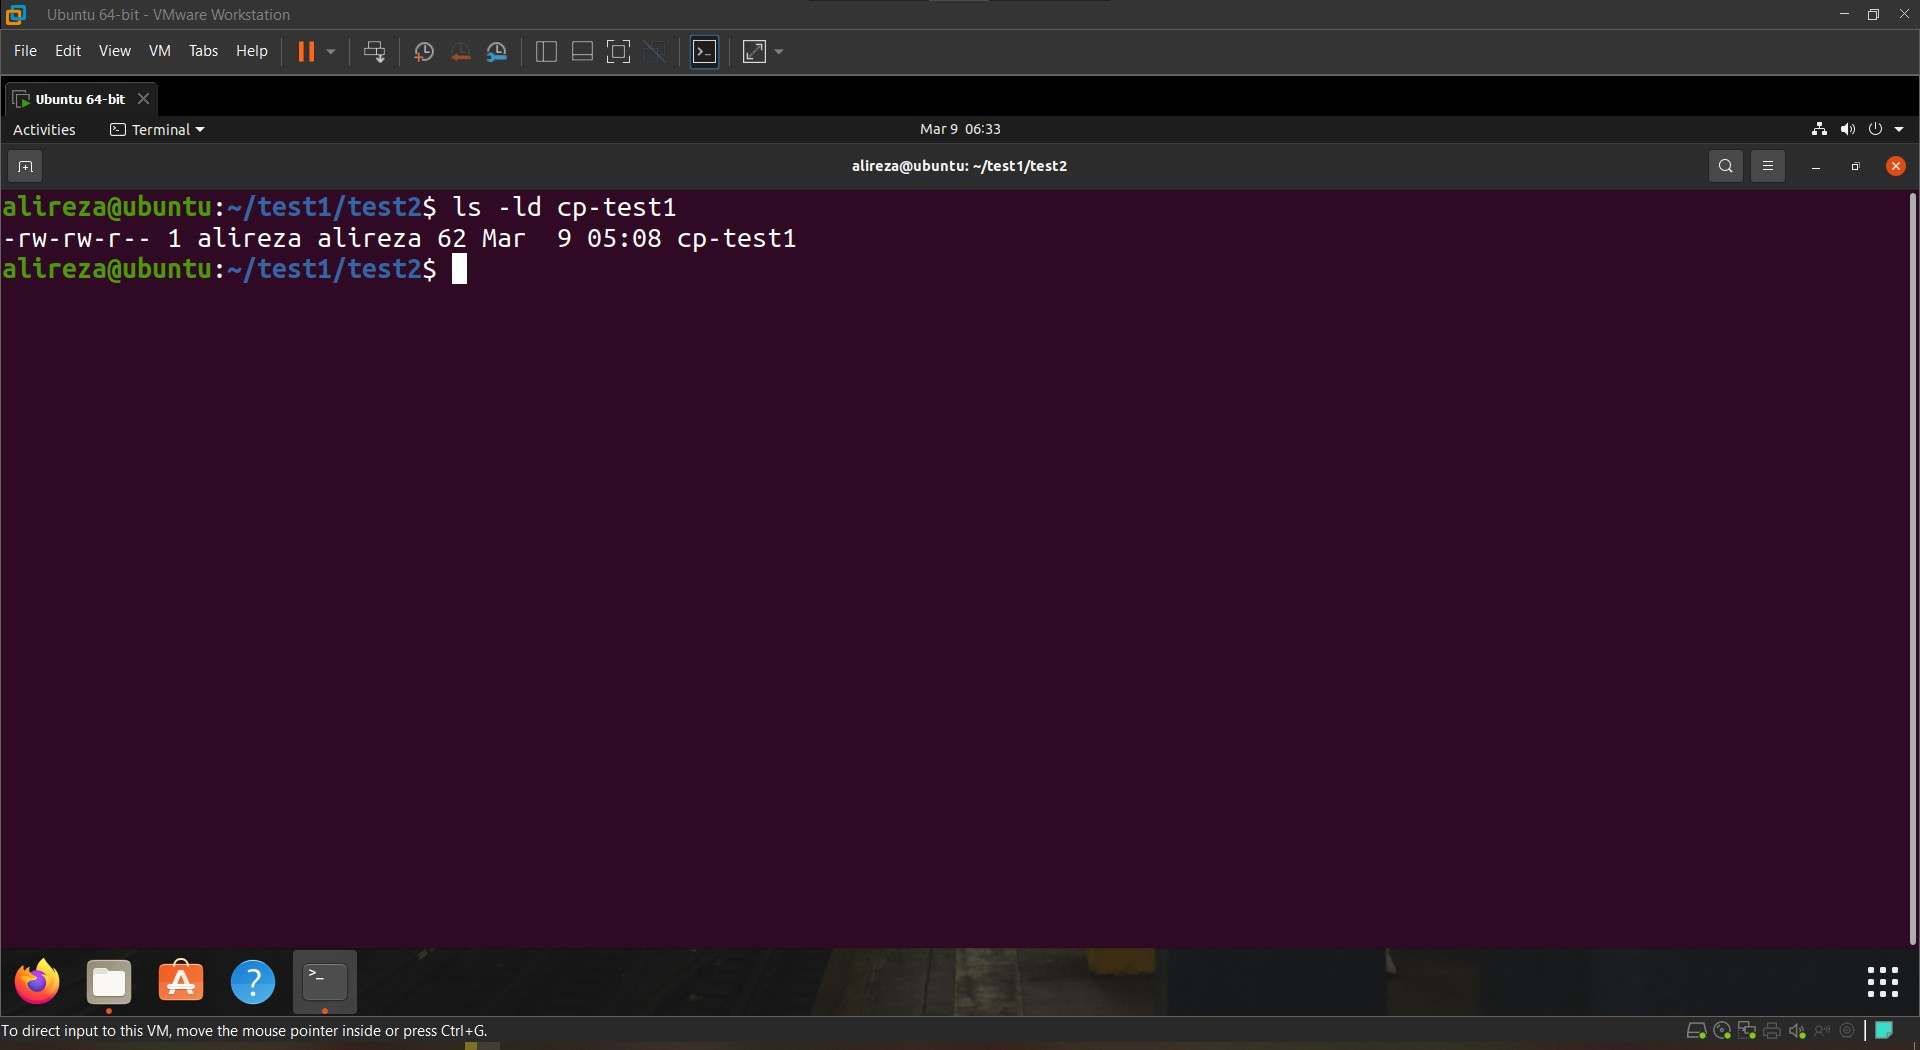
\includegraphics[width=1.0\textwidth]{figures/5a.jpg}
    \caption
	{
\lr{a}
	}
    \label{fig:fig1}
\end{figure}

\subsection{}
\begin{figure}[H]
    \centering
    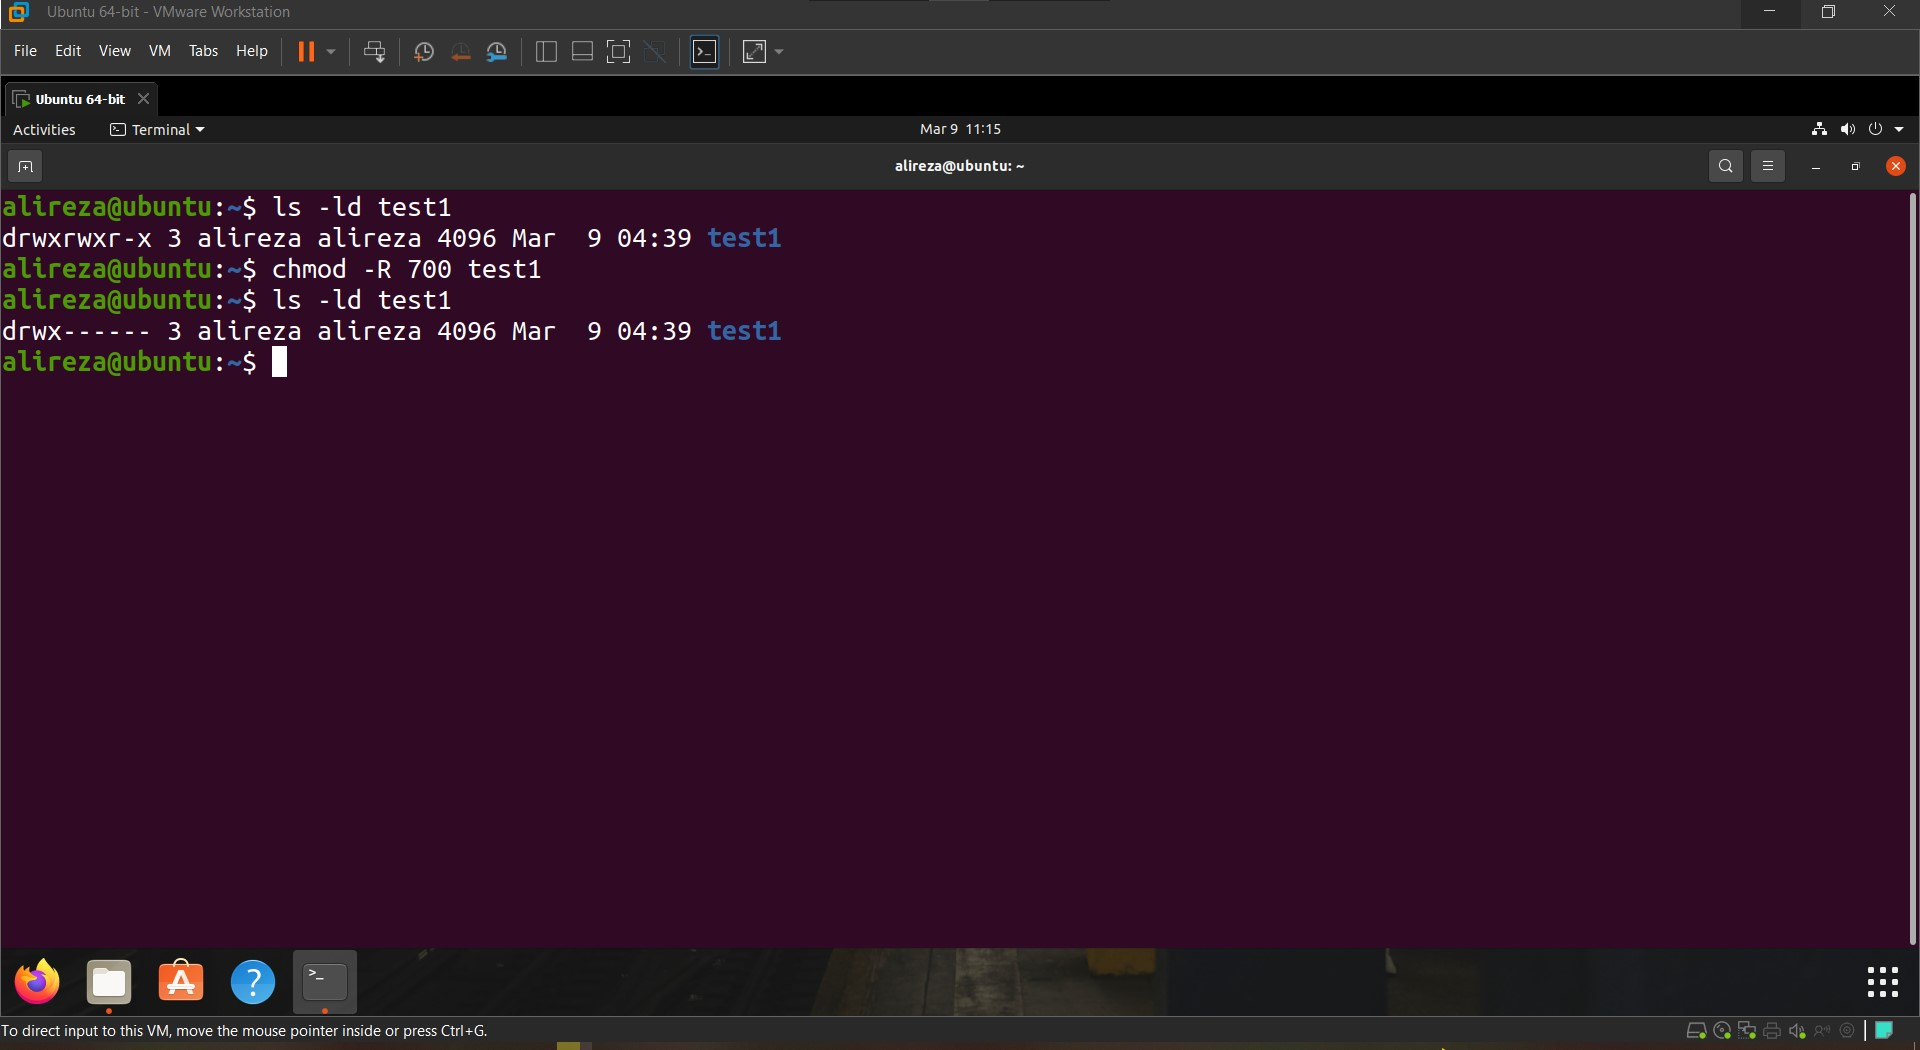
\includegraphics[width=1.0\textwidth]{figures/5b.jpg}
    \caption
	{
\lr{b}
	}
    \label{fig:fig1}
\end{figure}

\subsection{}
\begin{figure}[H]
    \centering
    
\includegraphics[width=1.0\textwidth]{figures/5c.jpg}
    \caption
	{
\lr{c}
	}
    \label{fig:fig1}
\end{figure}


\section{کار با محیط گرافیکی}
\begin{figure}[H]
    \centering
    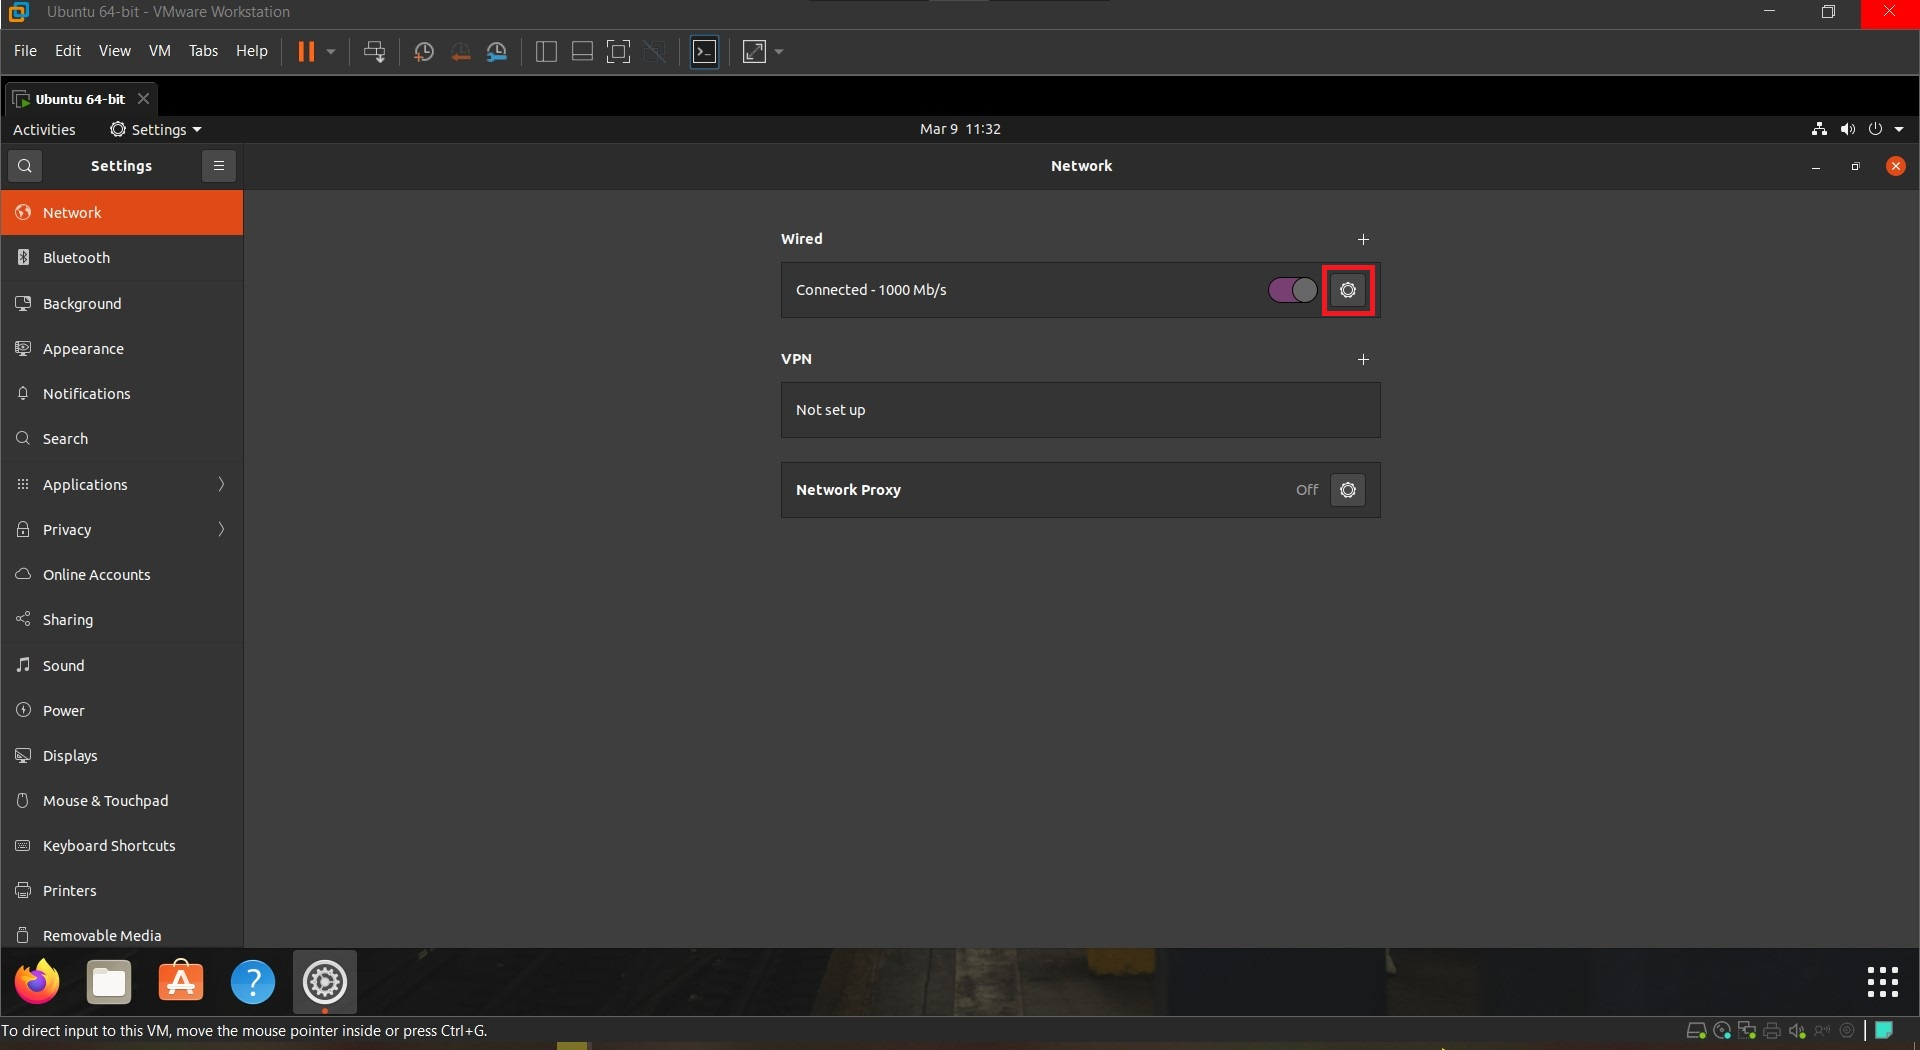
\includegraphics[width=1.0\textwidth]{figures/6a.jpg}
    \caption
	{
ورود به تنظیمات شبکه
	}
    \label{fig:fig1}
\end{figure}
\begin{figure}[H]
    \centering
    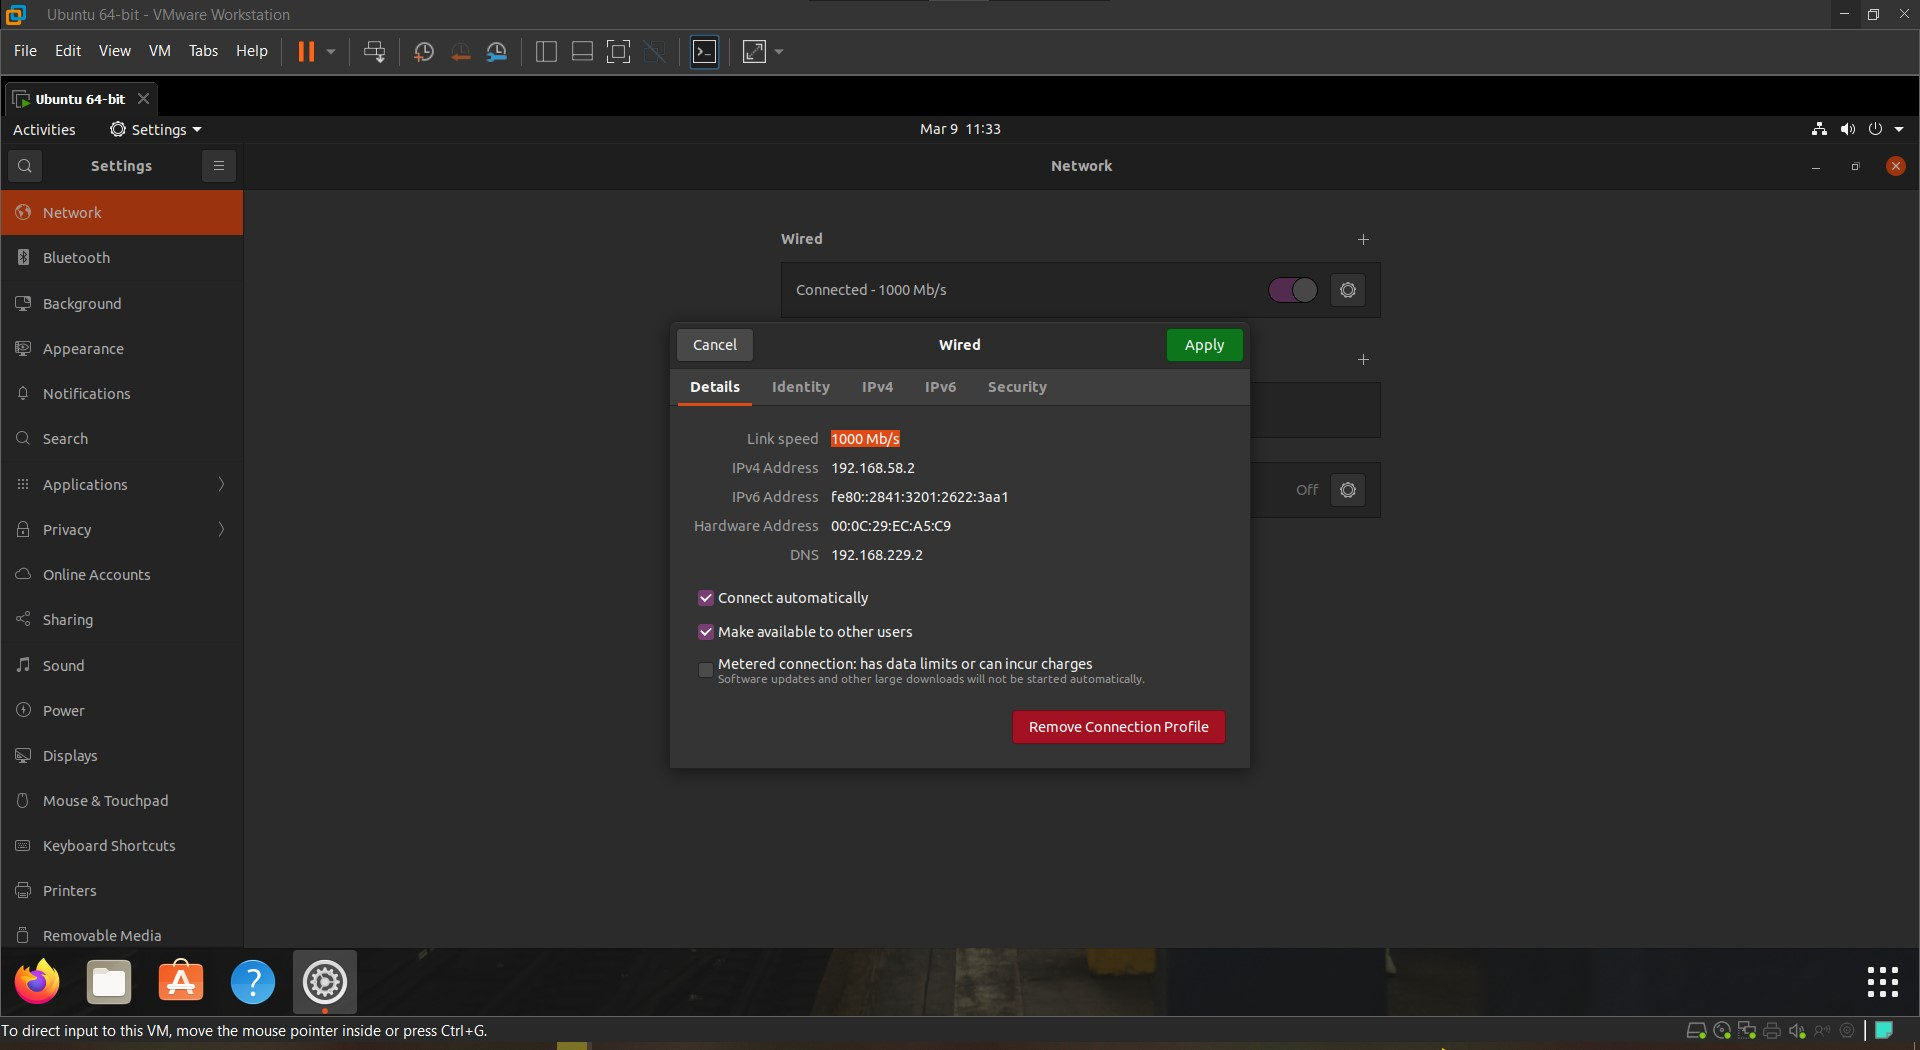
\includegraphics[width=1.0\textwidth]{figures/6b.jpg}
    \caption
	{
آدرس آی‌پی فعلی
	}
    \label{fig:fig1}
\end{figure}
\begin{figure}[H]
    \centering
    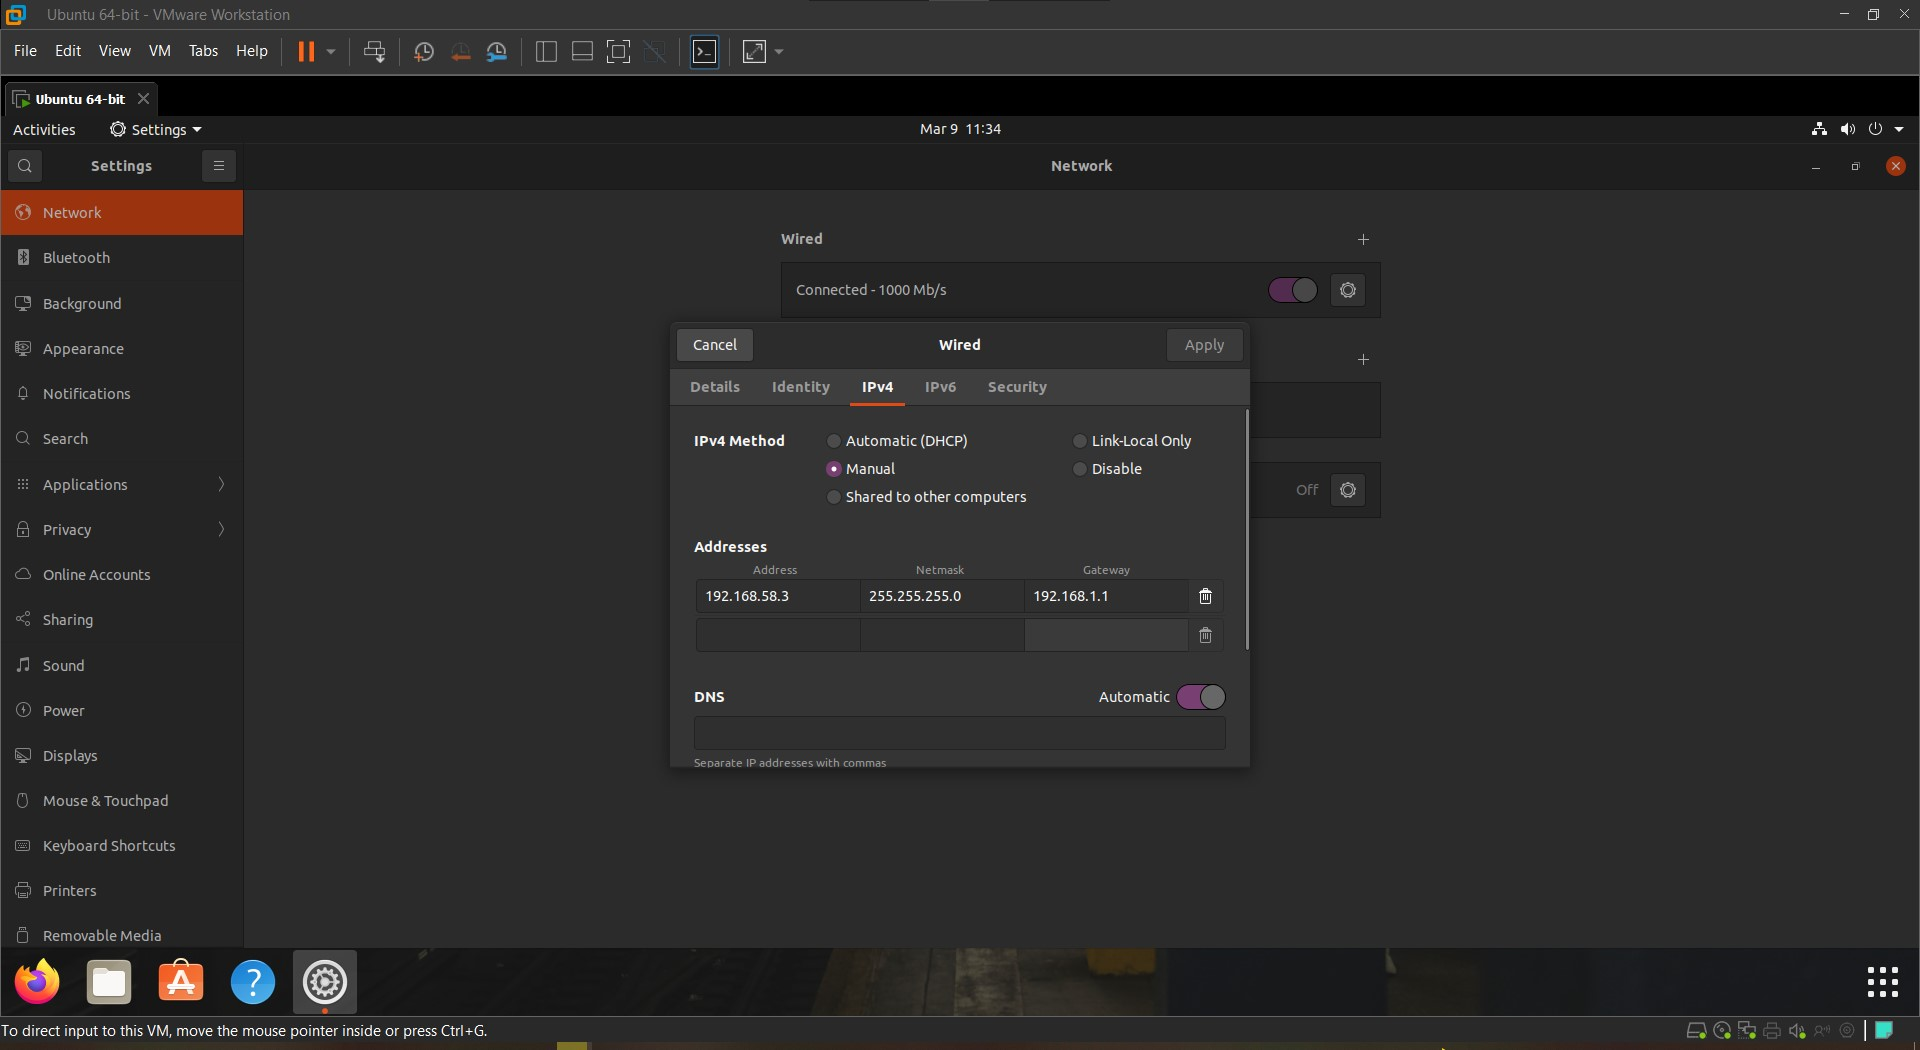
\includegraphics[width=1.0\textwidth]{figures/6c.jpg}
    \caption
	{
تغییر دستی آدرس آی‌پی
	}
    \label{fig:fig1}
\end{figure}
\begin{figure}[H]
    \centering
    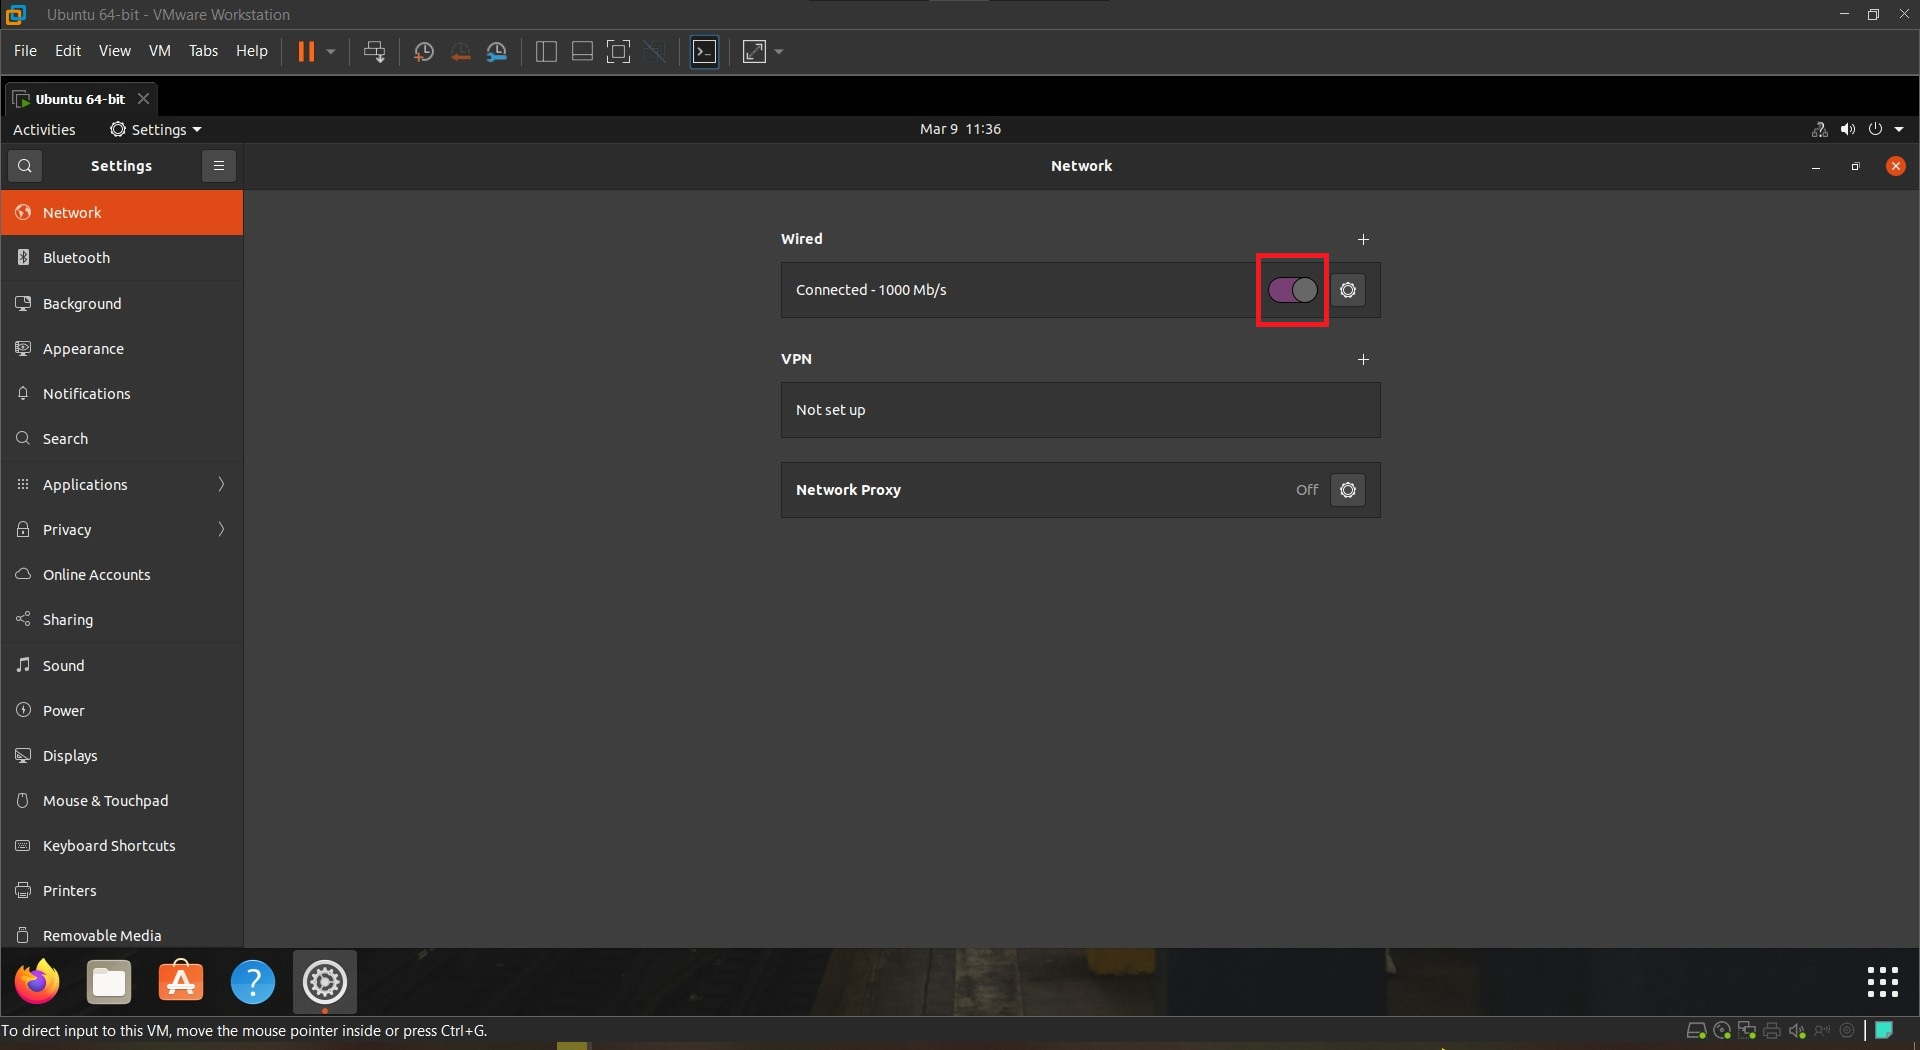
\includegraphics[width=1.0\textwidth]{figures/6d.jpg}
    \caption
	{
یک دور \lr{On/Off} می‌کنیم.
	}
    \label{fig:fig1}
\end{figure}
\begin{figure}[H]
    \centering
    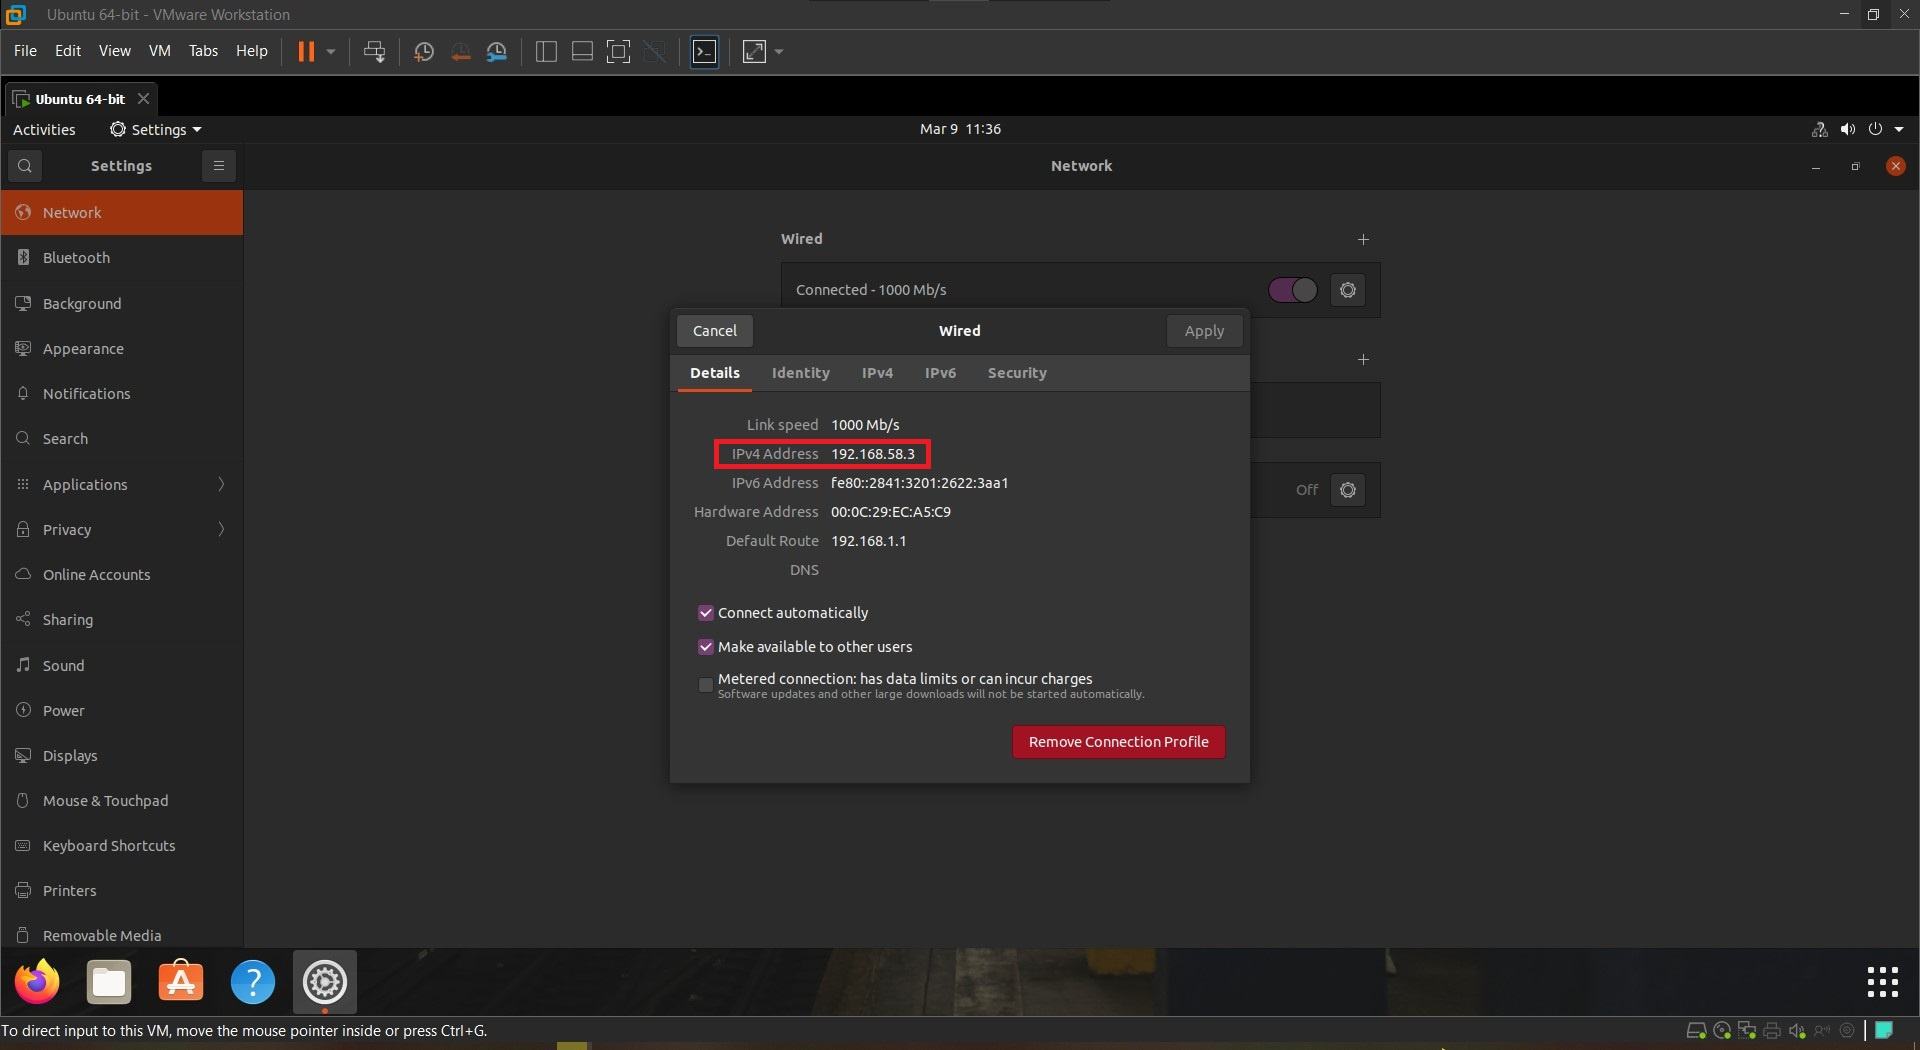
\includegraphics[width=1.0\textwidth]{figures/6e.jpg}
    \caption
	{
آدرس آی‌پی تغییر کرده است.
	}
    \label{fig:fig1}
\end{figure}


\section{تغییر آدرس آی‌پی از طریق خط فرمان}
\begin{figure}[H]
    \centering
    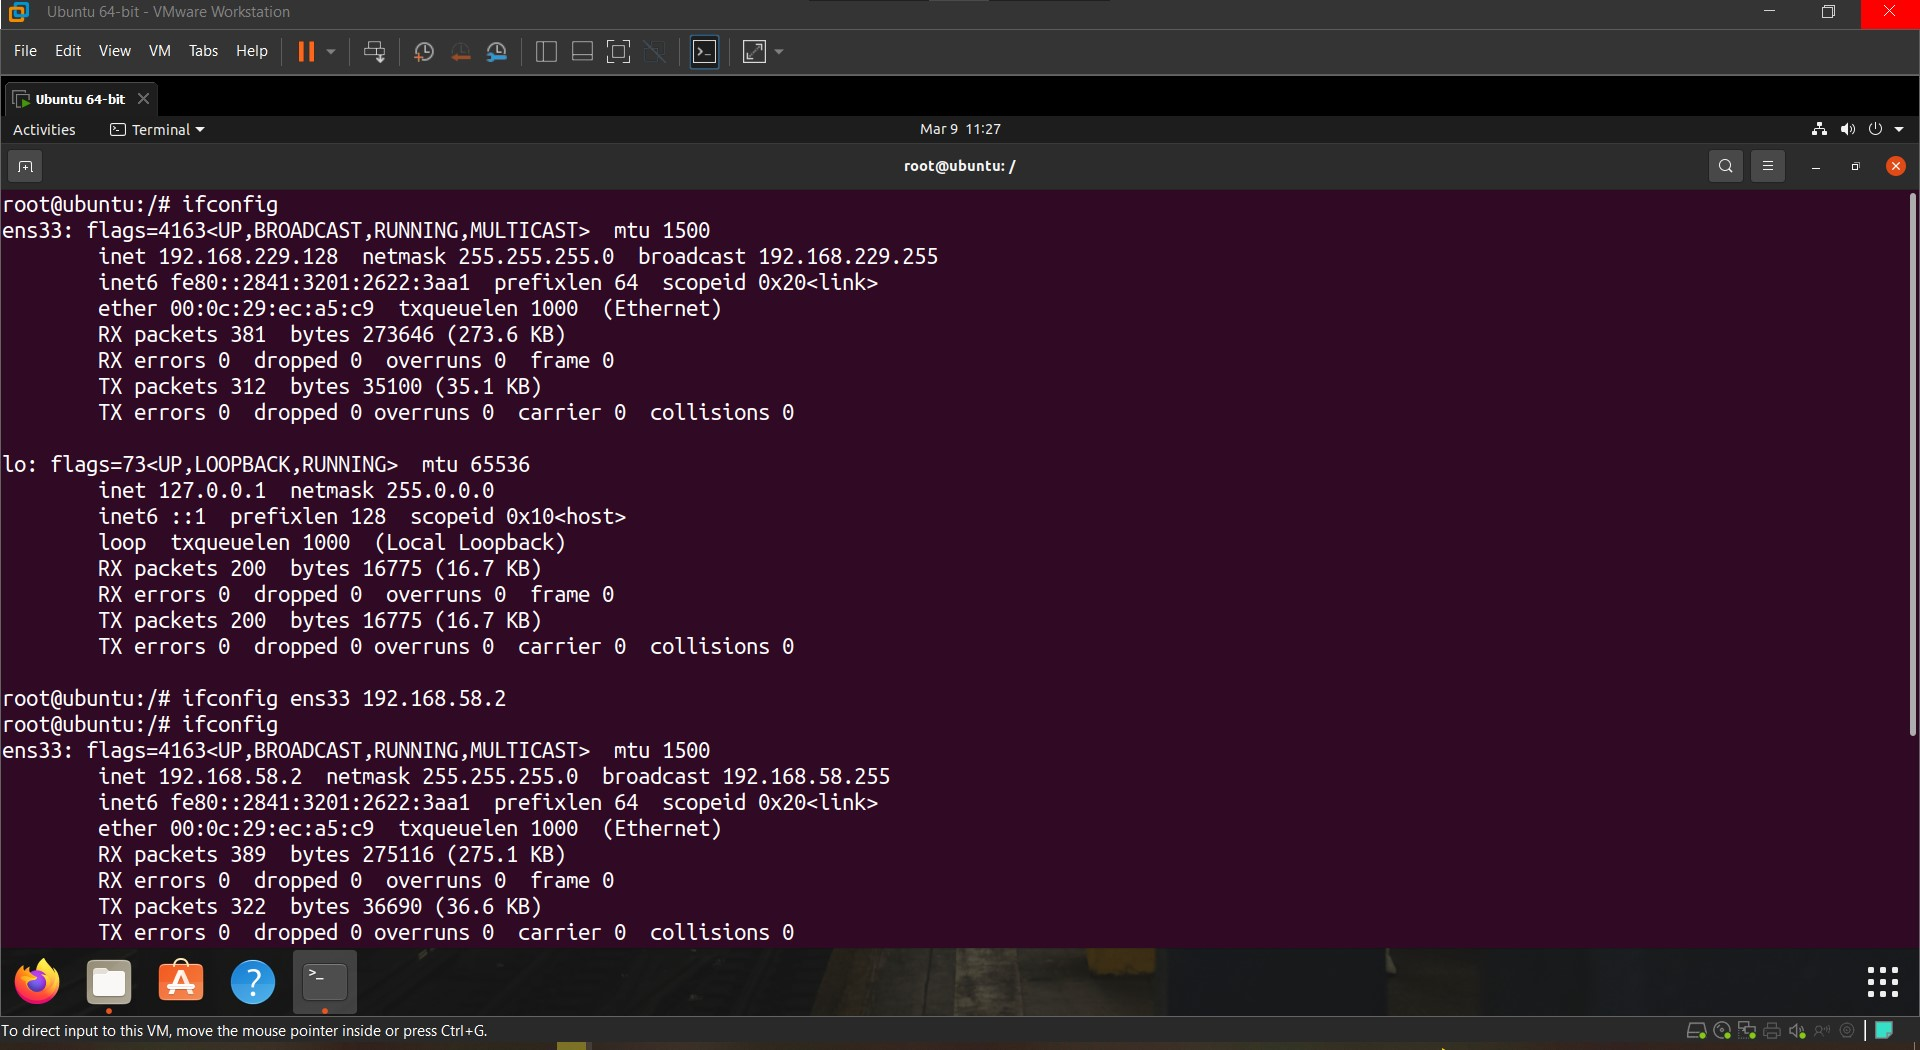
\includegraphics[width=1.0\textwidth]{figures/7.jpg}
    \caption
	{
تغییر آی‌پی به \lr{192.168.58.2}
	}
    \label{fig:fig1}
\end{figure}


\section{کار با دستور \lr{route}}
\subsection{}
\begin{figure}[H]
    \centering
    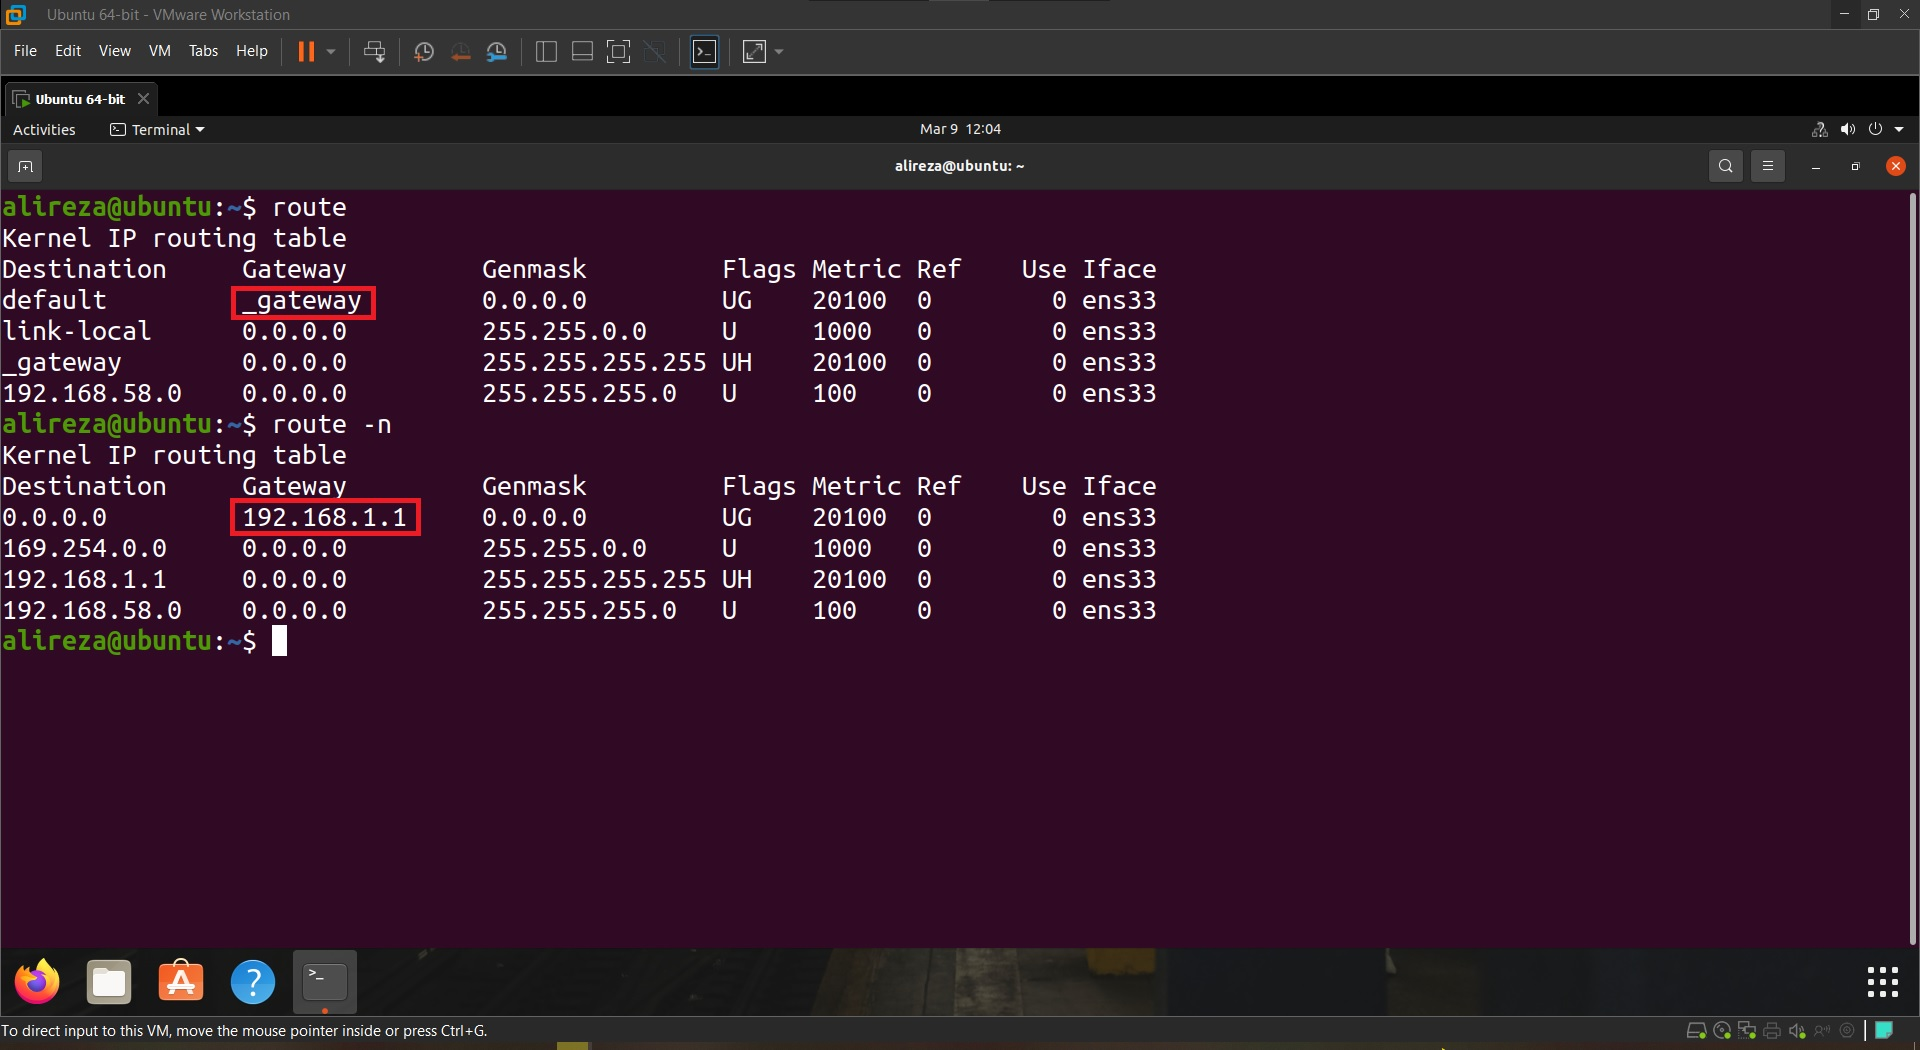
\includegraphics[width=1.0\textwidth]{figures/8a.jpg}
    \caption
	{
\lr{Default Gateway}
	}
    \label{fig:fig1}
\end{figure}

\subsection{}
\begin{figure}[H]
    \centering
    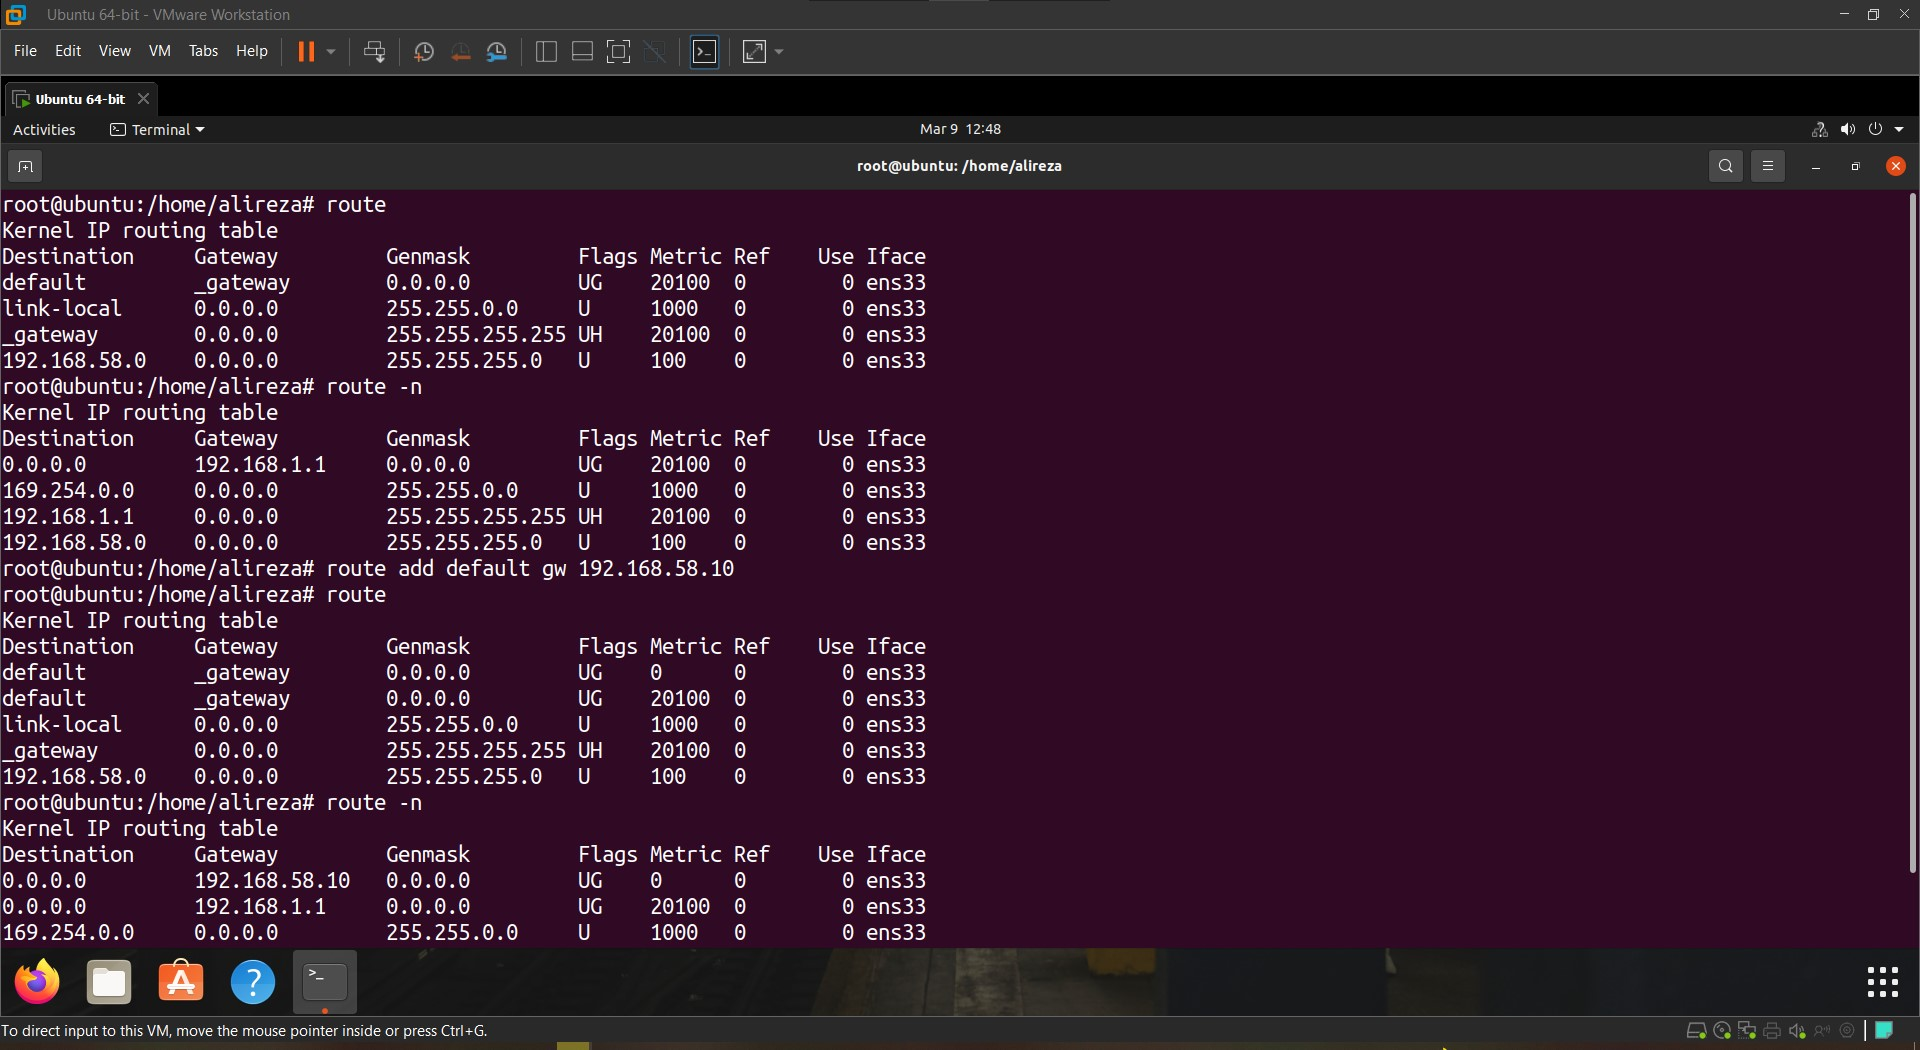
\includegraphics[width=1.0\textwidth]{figures/8b.jpg}
    \caption
	{
تغییر \lr{Default Gateway}
	}
    \label{fig:fig1}
\end{figure}

\subsection{}
\begin{figure}[H]
    \centering
    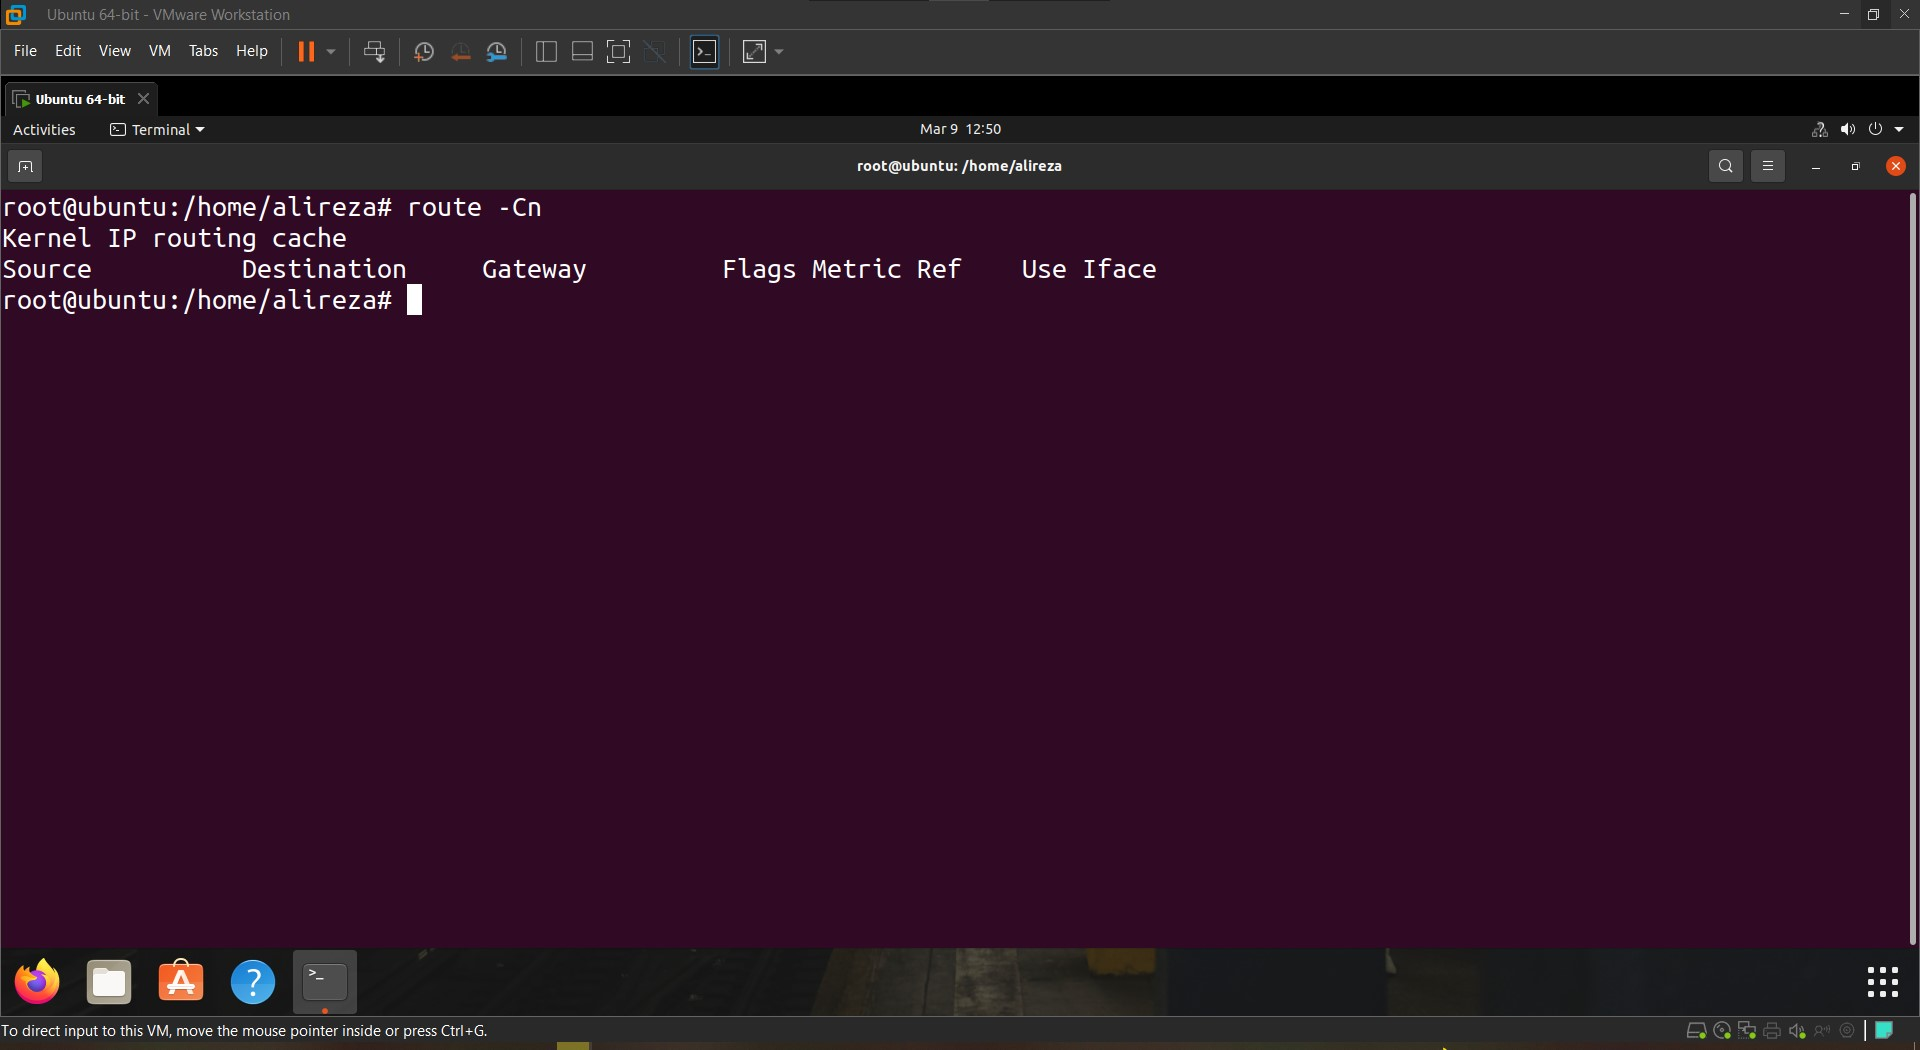
\includegraphics[width=1.0\textwidth]{figures/8c.jpg}
    \caption
	{
اطلاعات مسیریابی کش شده در سیستم
	}
    \label{fig:fig1}
\end{figure}

\subsection{}
اگر سیستمِ \lr{B} را در سیستمِ \lr{A} ریجکت کنیم، پینگ از دو طرف مسدود می‌شود. چون پینگ یک ارتباط دو طرفه است.


%%%%%%%%%%%%%%%%%%%%%%%%%%%%%%%%%%%%%%%%%%%%%%

\section*{منابع}
\renewcommand{\section}[2]{}%
\begin{thebibliography}{99} % assumes less than 100 references
%چنانچه مرجع فارسی نیز داشته باشید باید دستور فوق را فعال کنید و مراجع فارسی خود را بعد از این دستور وارد کنید


\begin{LTRitems}

\resetlatinfont

\bibitem{b1} 
\end{LTRitems}

\end{thebibliography}


\end{document}
